\documentclass[letterpaper,11pt]{article}
\usepackage{tabularx} % extra features for tabular environment
%\usepackage{amsmath}  % improve math presentation
\usepackage{graphicx} % takes care of graphic including machinery
\usepackage[margin=1in,letterpaper]{geometry} % decreases margins
\usepackage{subcaption}
%\usepackage{cite} % takes care of citations
%\usepackage{url}
\usepackage[final]{hyperref} % adds hyper links inside the generated pdf file
\hypersetup{
	colorlinks=true,       % false: boxed links; true: colored links
	linkcolor=blue,        % color of internal links
	citecolor=blue,        % color of links to bibliography
	filecolor=magenta,     % color of file links
	urlcolor=blue         
}
%\usepackage[backend=biber]{biblatex}
%\bibliography{bibItem.bib}{}
%\addbibresource{bibItem.bib}
%\bibliographystyle{plain}
\usepackage{blindtext}
\newcommand{\images}{images}
\newcommand{\fig}{Figure:}
%++++++++++++++++++++++++++++++++++++++++


\begin{document}

\begin{center}
{\Large Bypassing Tunnels: Leaking VPN Client Traffic by Abusing Routing Tables} 

{Nian Xue, New York University \\
Yashaswi Malla, Zihang Xia, Christina Pöpper, New York University Abu Dhabi\\
Mathy Vanhoef, imec-DistriNet, KU Leuven}
\bigskip

{\large Writer: Akib Jawad Nafis}
\date{\today}
\end{center}


%\section{Summary}
%
%Your summary goes here 
%
%%\blindtext %delete this line
%
%
%\section{Strengths and Weaknesses}
%
%3-Key points for strengths and weaknesses each.
%
%%\blindtext % delete this line

\section{Introduction}
VPN (Virtual Private Network) has been widely used for a for security and privacy both in personal and professional setting.
VPNs encrypt network packets to protect user's privacy and
ensure secure access to internal resources for employees when they are working remotely.
A study \cite{vpnleaks} published by researchers actually built two attacks to bypass VPNs encryption.
On both of those attacks, researchers manipulated the routing table to bypass VPNs encryption and
leak user traffic outside of the VPN tunnel.
Goal of this project was to reproduce the attack scenarios proposed in the study \cite{vpnleaks}.

\section{How VPNs Work?}
VPNs operate by creating a virtual network interface called tun device.
After that VPN client application modifies the routing table of user device in way so that all network is sent to the tun interface.
Inside the tun interface it will encrypt the network packet and repackage the encrypted network packet
so that encrypted packet in sent to the VPN server. 
To keep functionality of the network, traffic to VPN server must not be encrypted. 
Therefore in the routing table, VPN client creates an exception for the VPN server's network.
Additionally, to keep access to any service running local network, VPN client also add another exception for traffic to local network.
\fig \ref{fig:routing} presents the state of the routing table when VPN is enabled.

\begin{figure}[h]
	\centering
	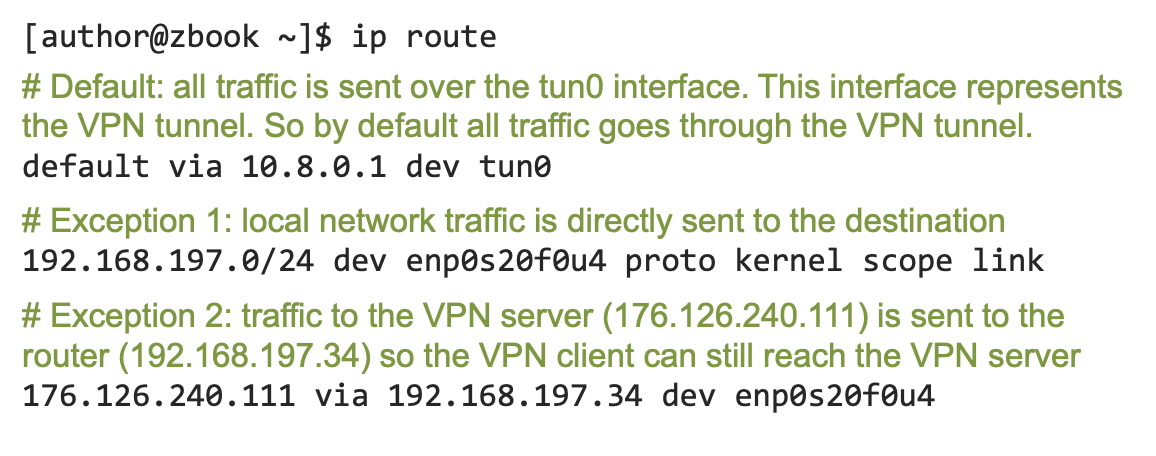
\includegraphics[width=\linewidth]{\images/routing_table_vpn}
	\caption{Routing Table with VPN enabled}
	\label{fig:routing}
\end{figure}

\section{Manipulation of Routing Exceptions: Attacks}
Due to the network route exceptions, packets from user device can flow outside of the VPN tunnel.
If traffic to any server which is neither the VPN server nor local network can be sent through these exception routes,
then purpose of using VPN will be nullified. Authors of the paper \cite{vpnleaks} built two attacks to send traffic to any specific website through the unencrypted routes.

\subsection{LocalNet Attack} In this attack, routing exception to local network is abused to send traffic to a target website via unencrypted channel. Here authors setup a rouge access point which will distrubute an ip address from the subnet of the target website.
As a result user's device will think the target website is in the local network. Hence traffic to target network will be sent through unencrypted channel, bypassing the VPN tunnel. \fig \ref{fig:localnet} presents the attack and \fig \ref{fig:localnetdetails} presents steps to carry out local net attack for target.com.

\begin{figure*}[h]
	\centering
	\begin{subfigure}{0.42\textwidth}
		\centering
		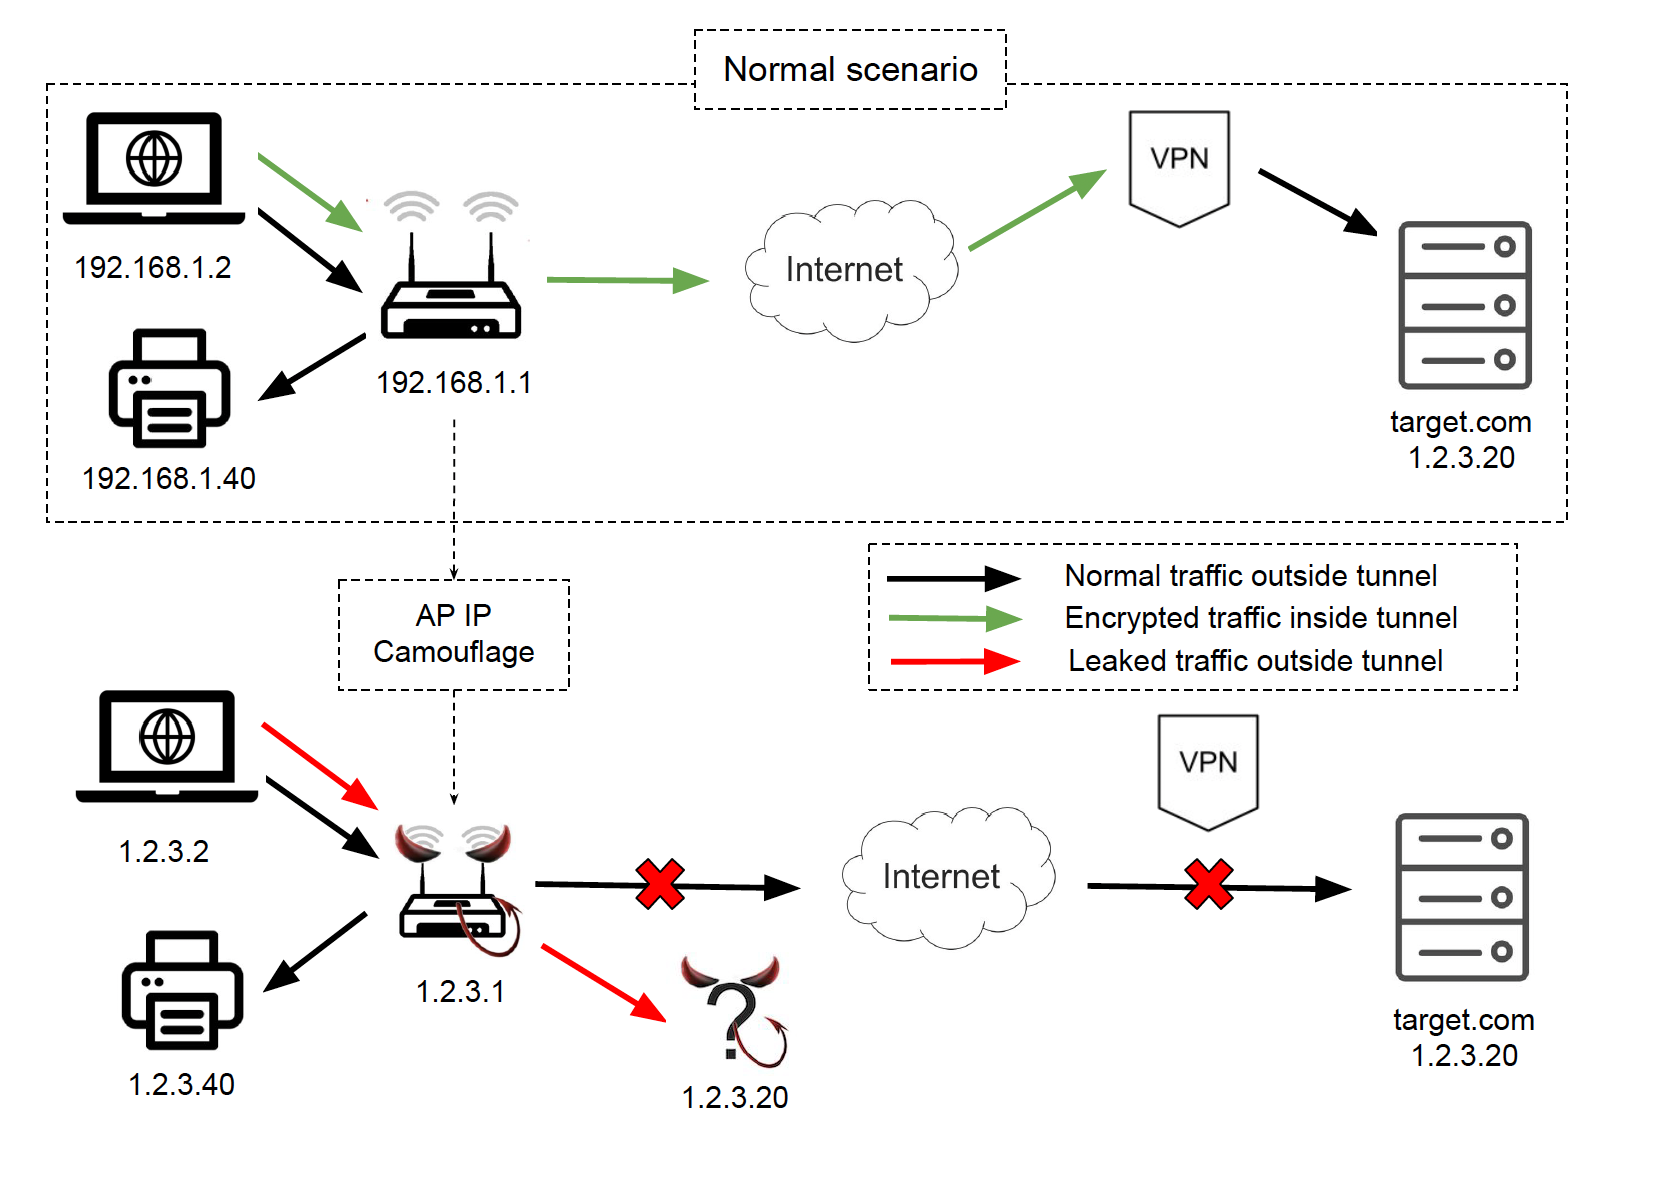
\includegraphics[width=\linewidth]{\images/LocalNetAttack}
		\caption{Local net attack using rouge access points}
		\label{fig:localnet}
	\end{subfigure}
	\begin{subfigure}{0.56\textwidth}
		\centering
		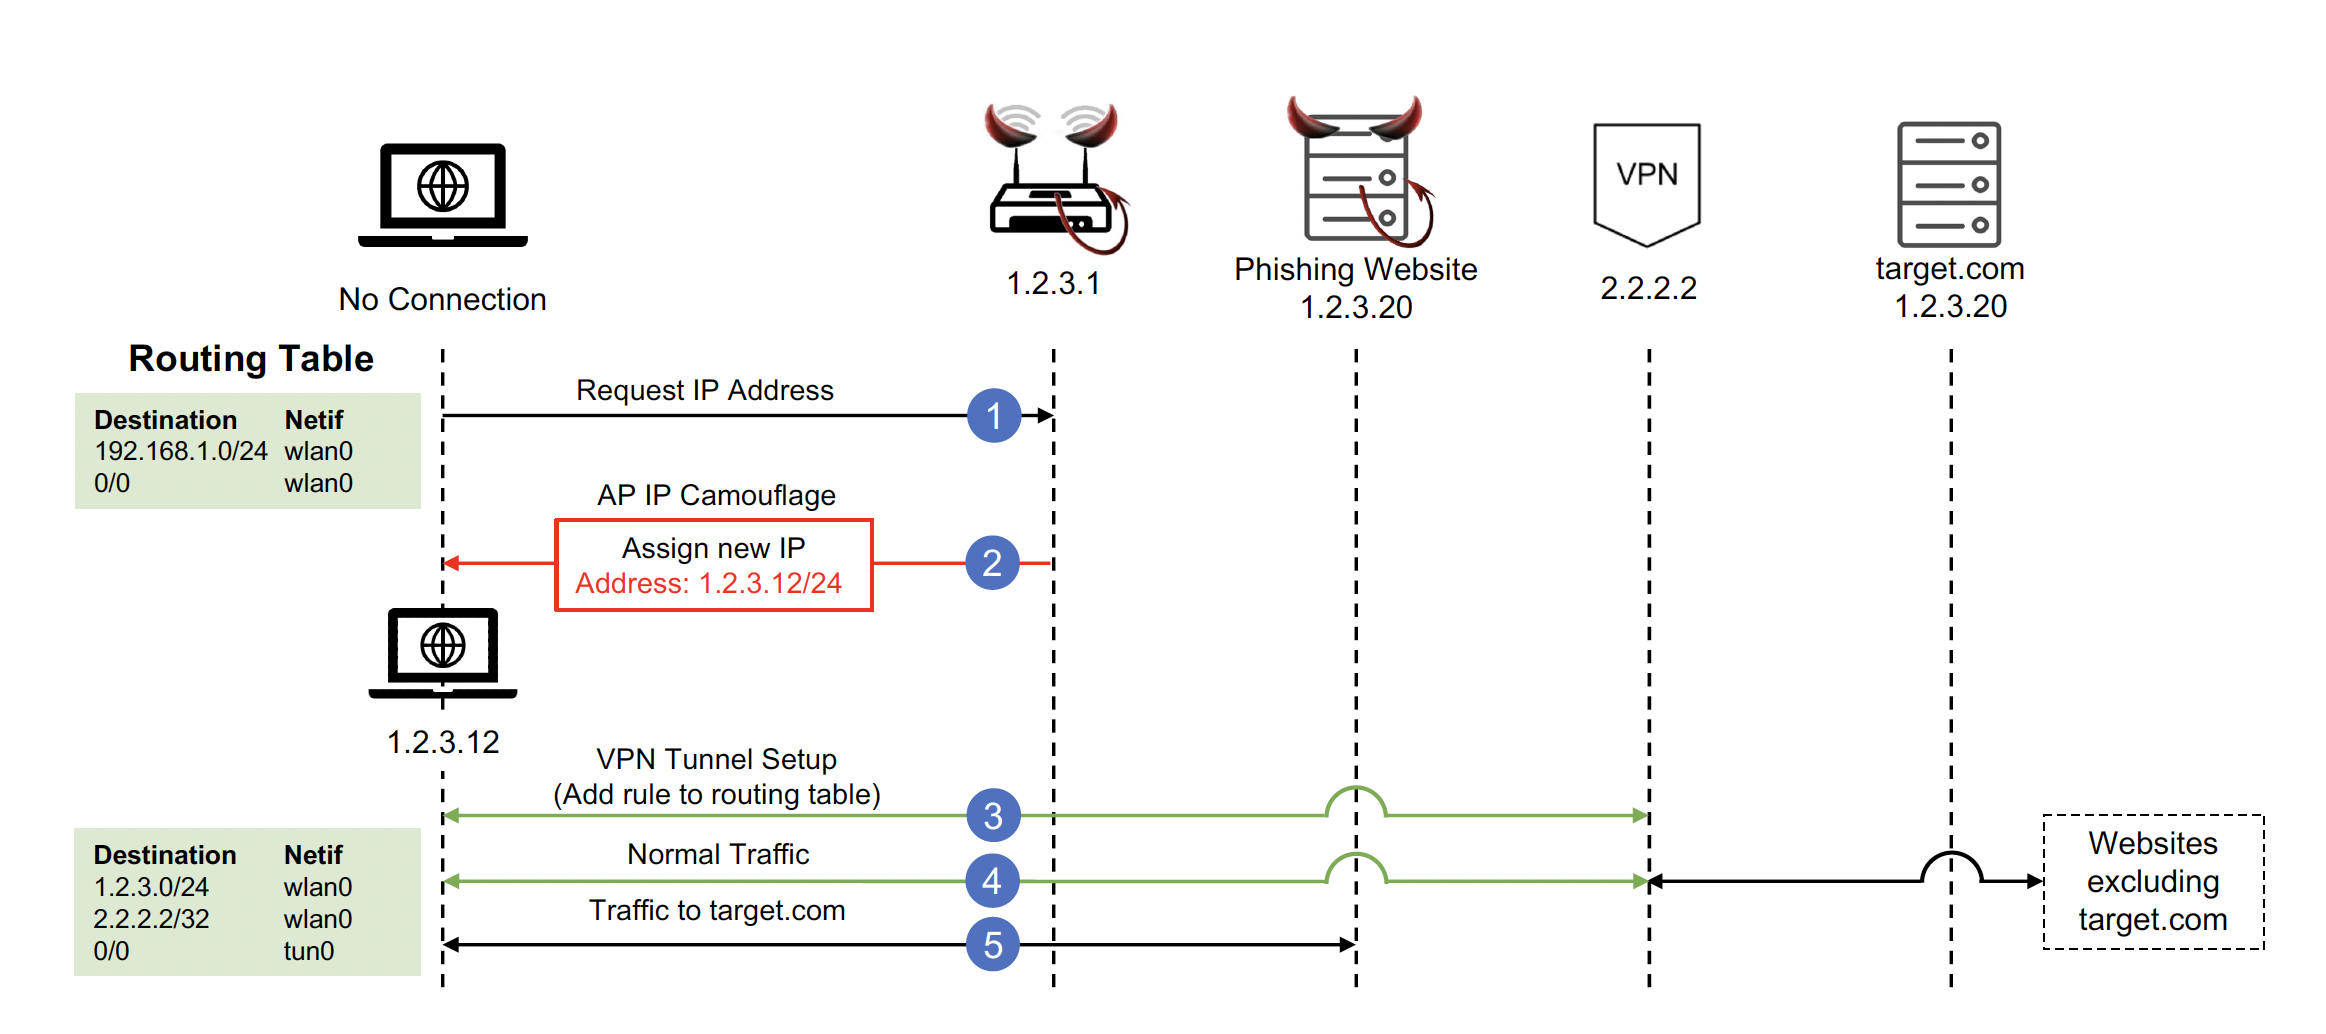
\includegraphics[width=\linewidth]{\images/Local-Net-Attack-details}
		\caption{Steps to carry out local net attack}
		\label{fig:localnetdetails}
	\end{subfigure}
	\caption{Formation of LocalNet Attack}
\end{figure*}




\subsection{ServerIP Attack}
In this attack, routing exception for traffic to VPN server will be misused to leak traffic to target website outside of the VPN tunnel.
In this case, rogue access point will work as a malicious DNS server.
During the VPN tunnel setup, user's device, which is connected to the rogue access point, will ask for the IP address of the VPN server.
Then malicious DNS server in the rouge access point will send the IP address of the target website as the IP address of the VPN server.
As a result, user's device will think traffic to target website is traffic to VPN server. 
Hence, it will send the traffic through the exception route to the VPN server. 
As a result, traffic to target website will be sent outside of the encrypted VPN tunnel.
\fig \ref{fig:serverip} presents the ServerIP attack and \fig \ref{fig:serveripattackdetails} shows the steps to carry out ServerIP-Attack.

\begin{figure*}
	\begin{subfigure}{0.42\textwidth}
		\centering
		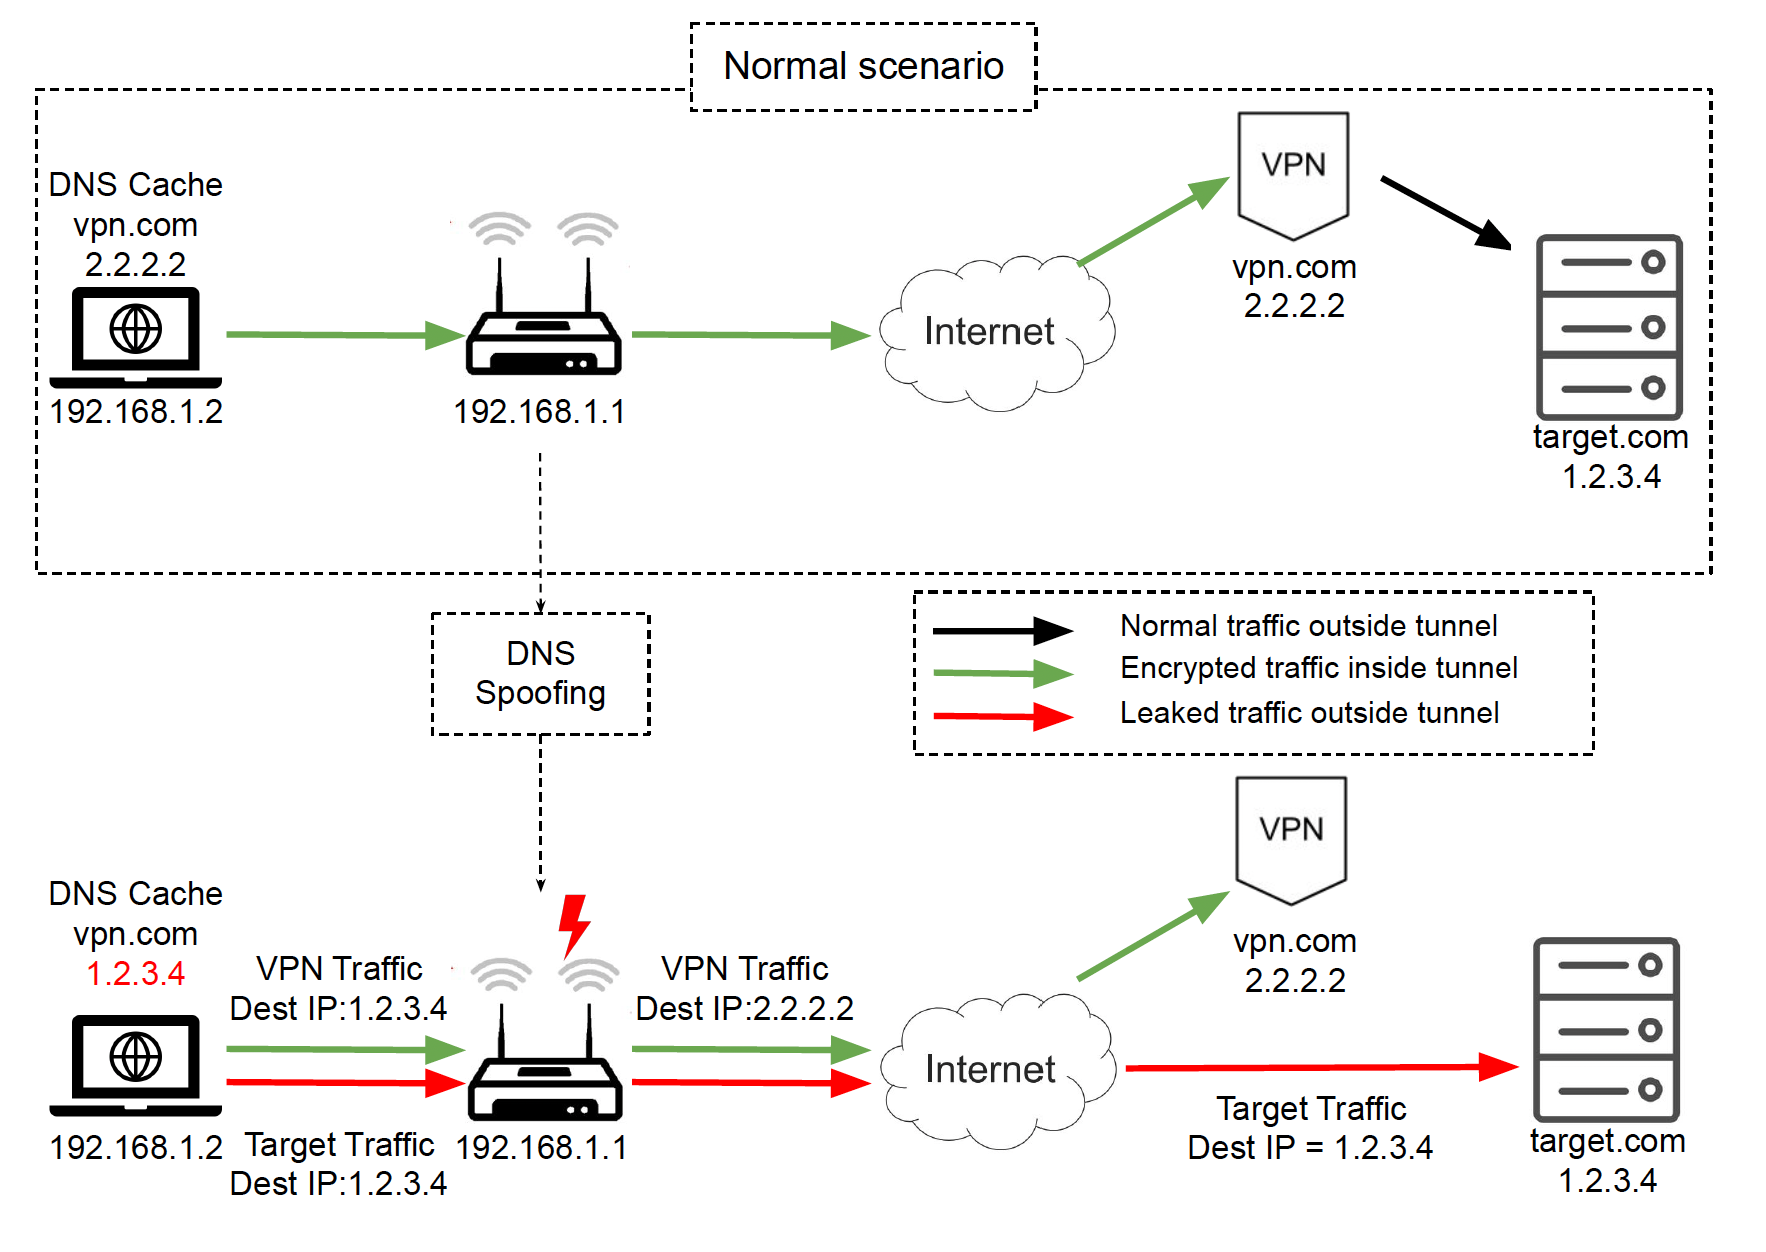
\includegraphics[width=\linewidth]{\images/ServerIP-Attack}
		\caption{Server IP attack using rouge access points}
		\label{fig:serverip}
	\end{subfigure}
	\begin{subfigure}{0.56\textwidth}
		\centering
		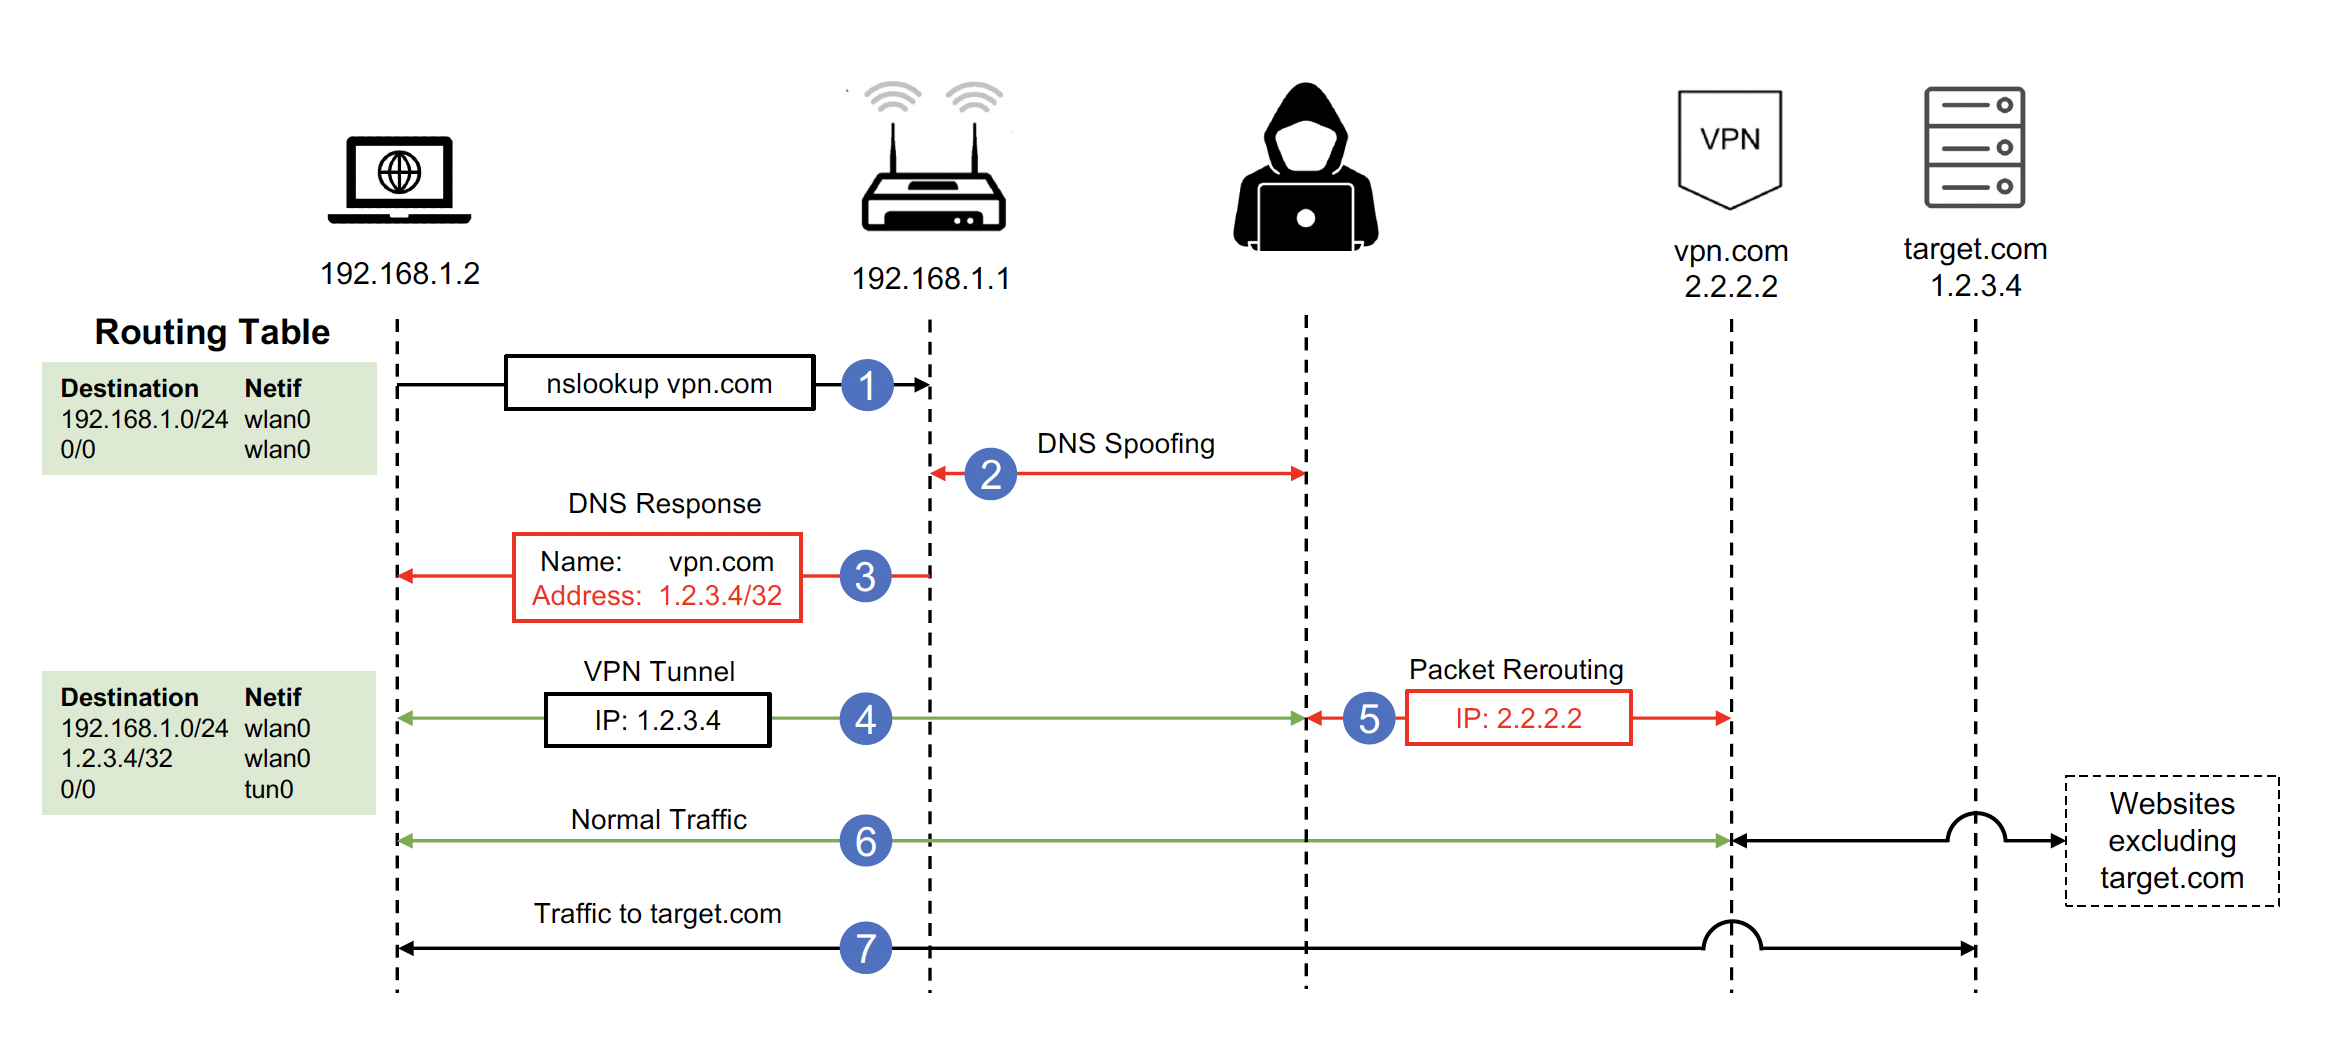
\includegraphics[width=\linewidth]{\images/ServerNet-Attack-details}
		\caption{Steps to carry out ServerIP attack}
		\label{fig:serveripattackdetails}
	\end{subfigure}
	\caption{Formation of ServerIP Attack}
\end{figure*}

%\begin{figure}[h]
%	\centering
%	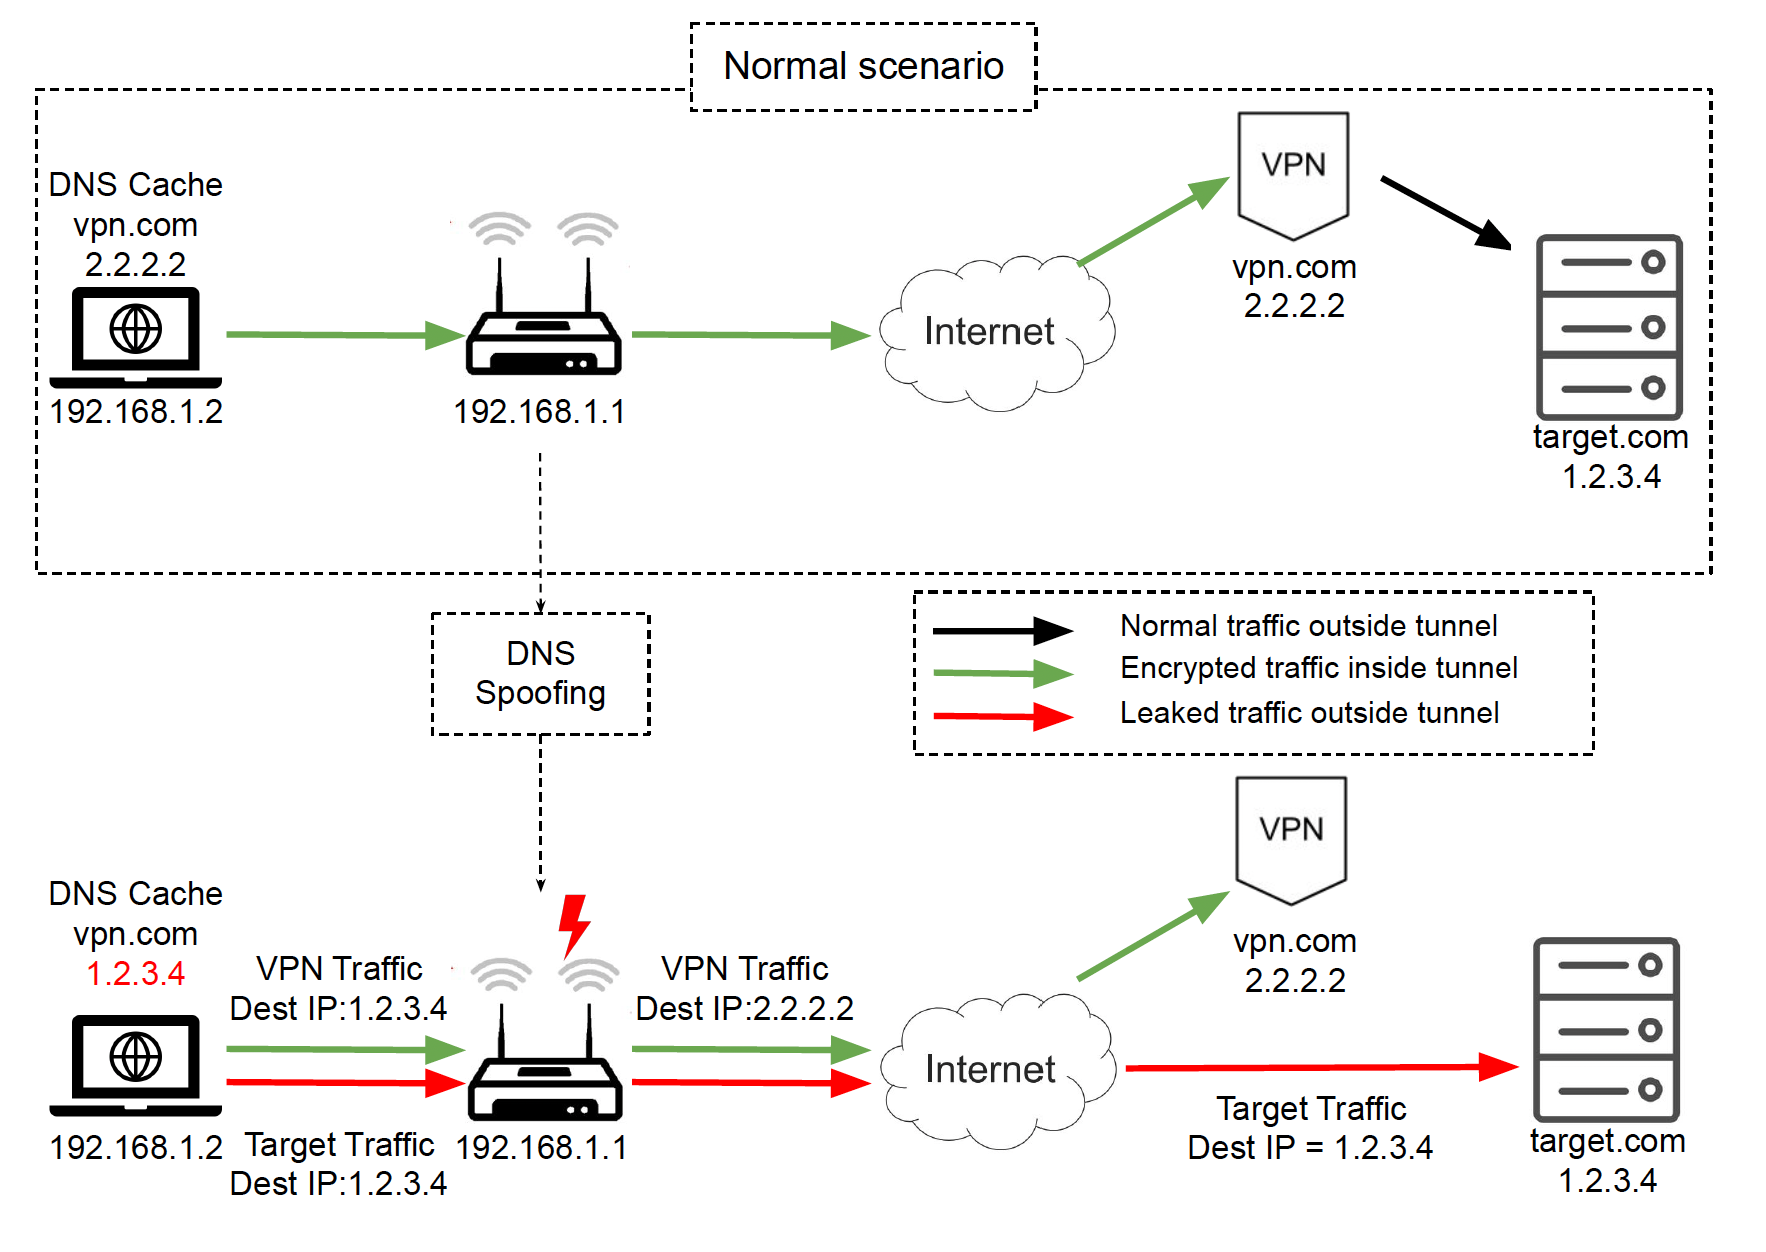
\includegraphics[width=\linewidth]{\images/ServerIP-Attack}
%	\caption{Server IP attack using rouge access points}
%	\label{fig:serverip}
%\end{figure}

%\begin{figure}[h]
%	\centering
%	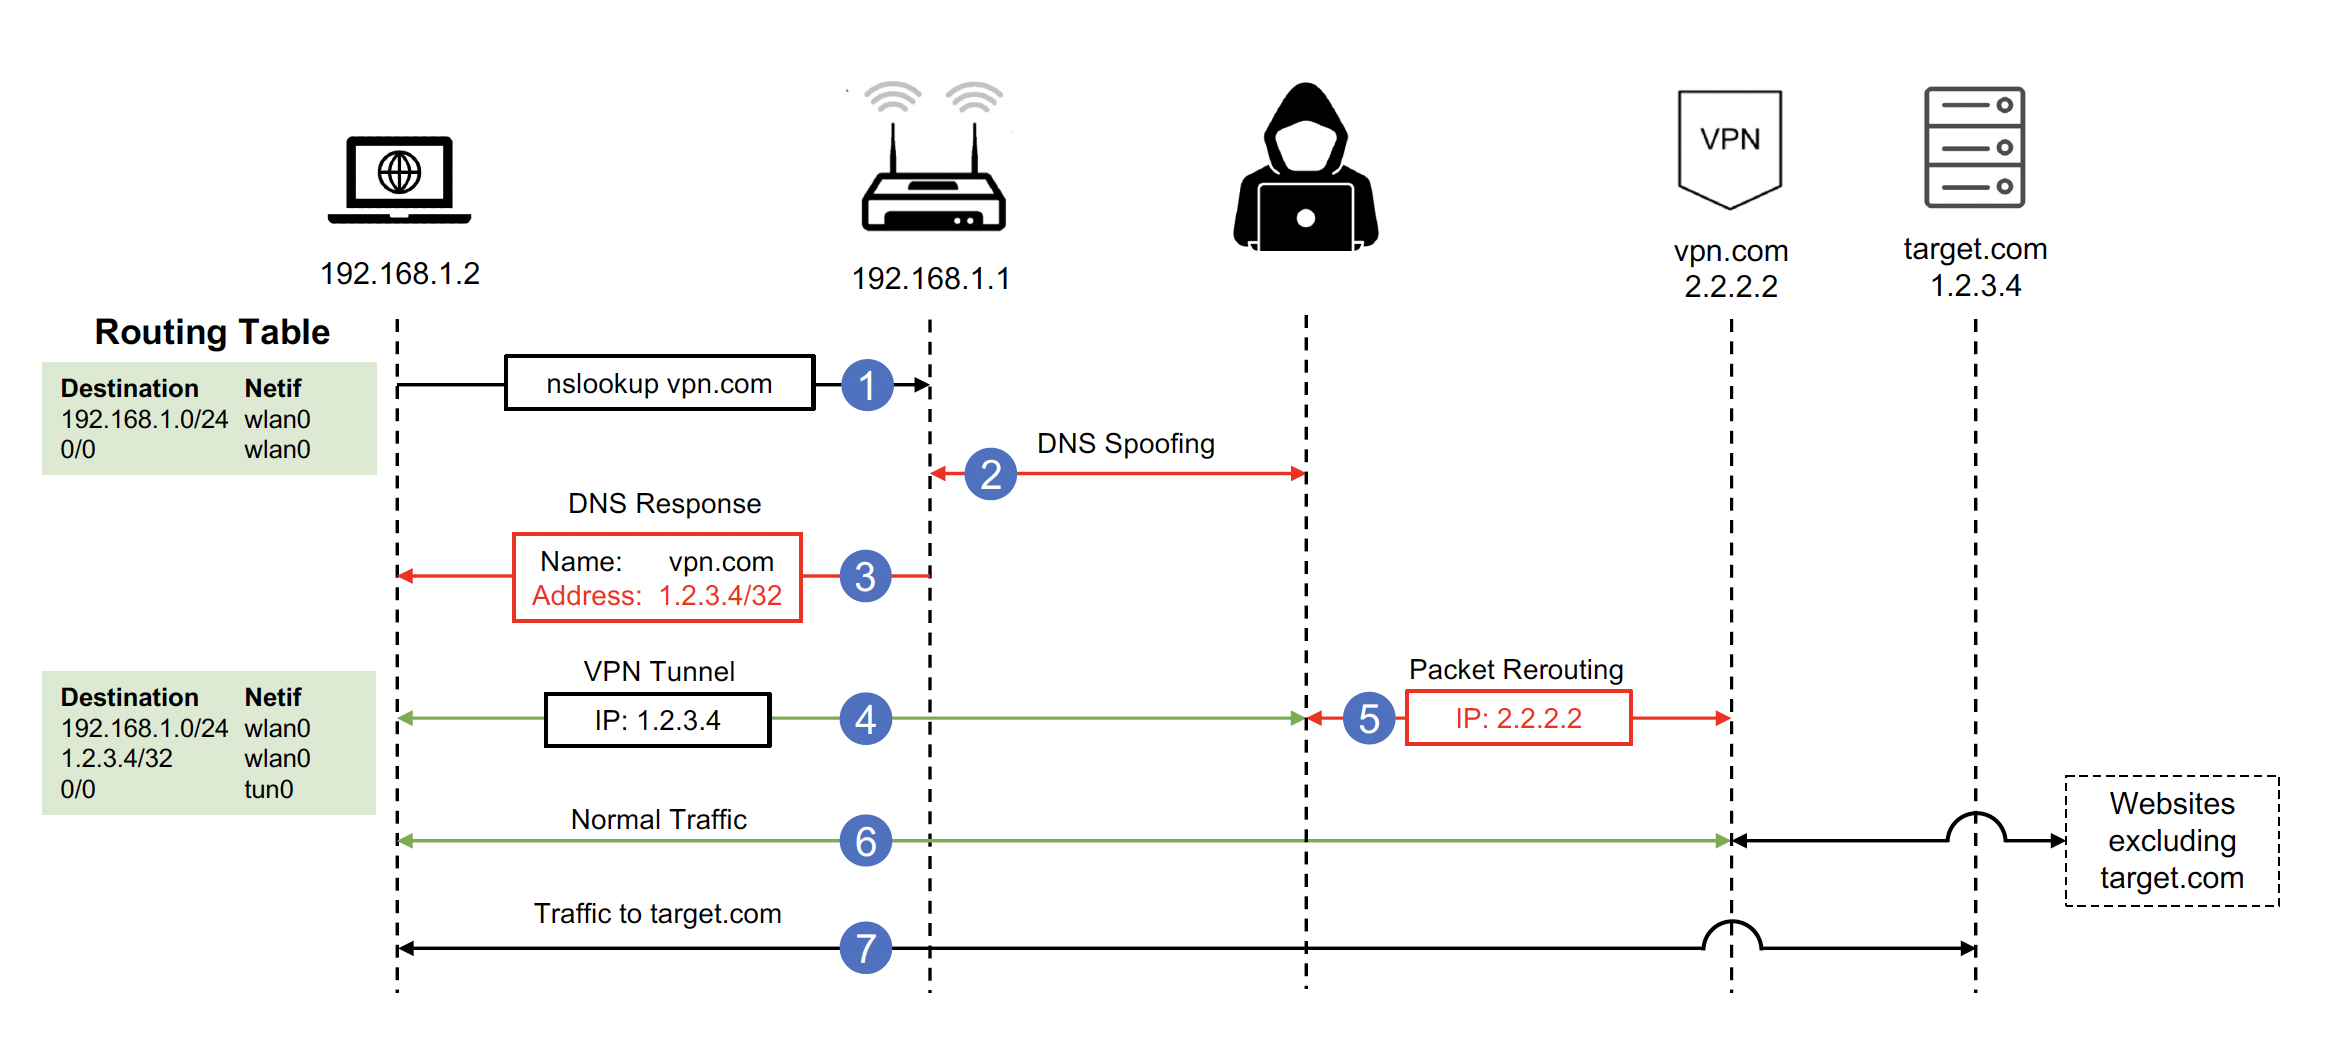
\includegraphics[width=\linewidth]{\images/ServerNet-Attack-details}
%	\caption{Steps to carry out ServerIP attack}
%	\label{fig:serveripattackdetails}
%\end{figure}

\section{Experimental Setup}

To reproduce the attack developed in the paper \cite{vpnleaks}, I set up my environment following the description given in the paper.
\fig \ref{fig:local-net-setup} shows my setup for LocalNet attack.
To create a rogue access point I used a Panda PAU04 network card \cite{panda} and create\_ap script \cite{createap}.
For the LocalNet attack, I set up an aws server to have a target website which just runs a nginx server \cite{nginx}.
This is a public server with the IP address 35.164.87.16.
I also created a local clone of the server with the same IP address to catch when LocalNetAttack is successful.
The local server also runs nginx server, but on the home page it says "CLONE". 
When user's device is using VPN and user is visiting the target website 35.164.87.16, if user device shows the local webpage with ``CLONE'' in it, we can confirm that VPN client is leaking.

\begin{figure}[h]
	\centering
	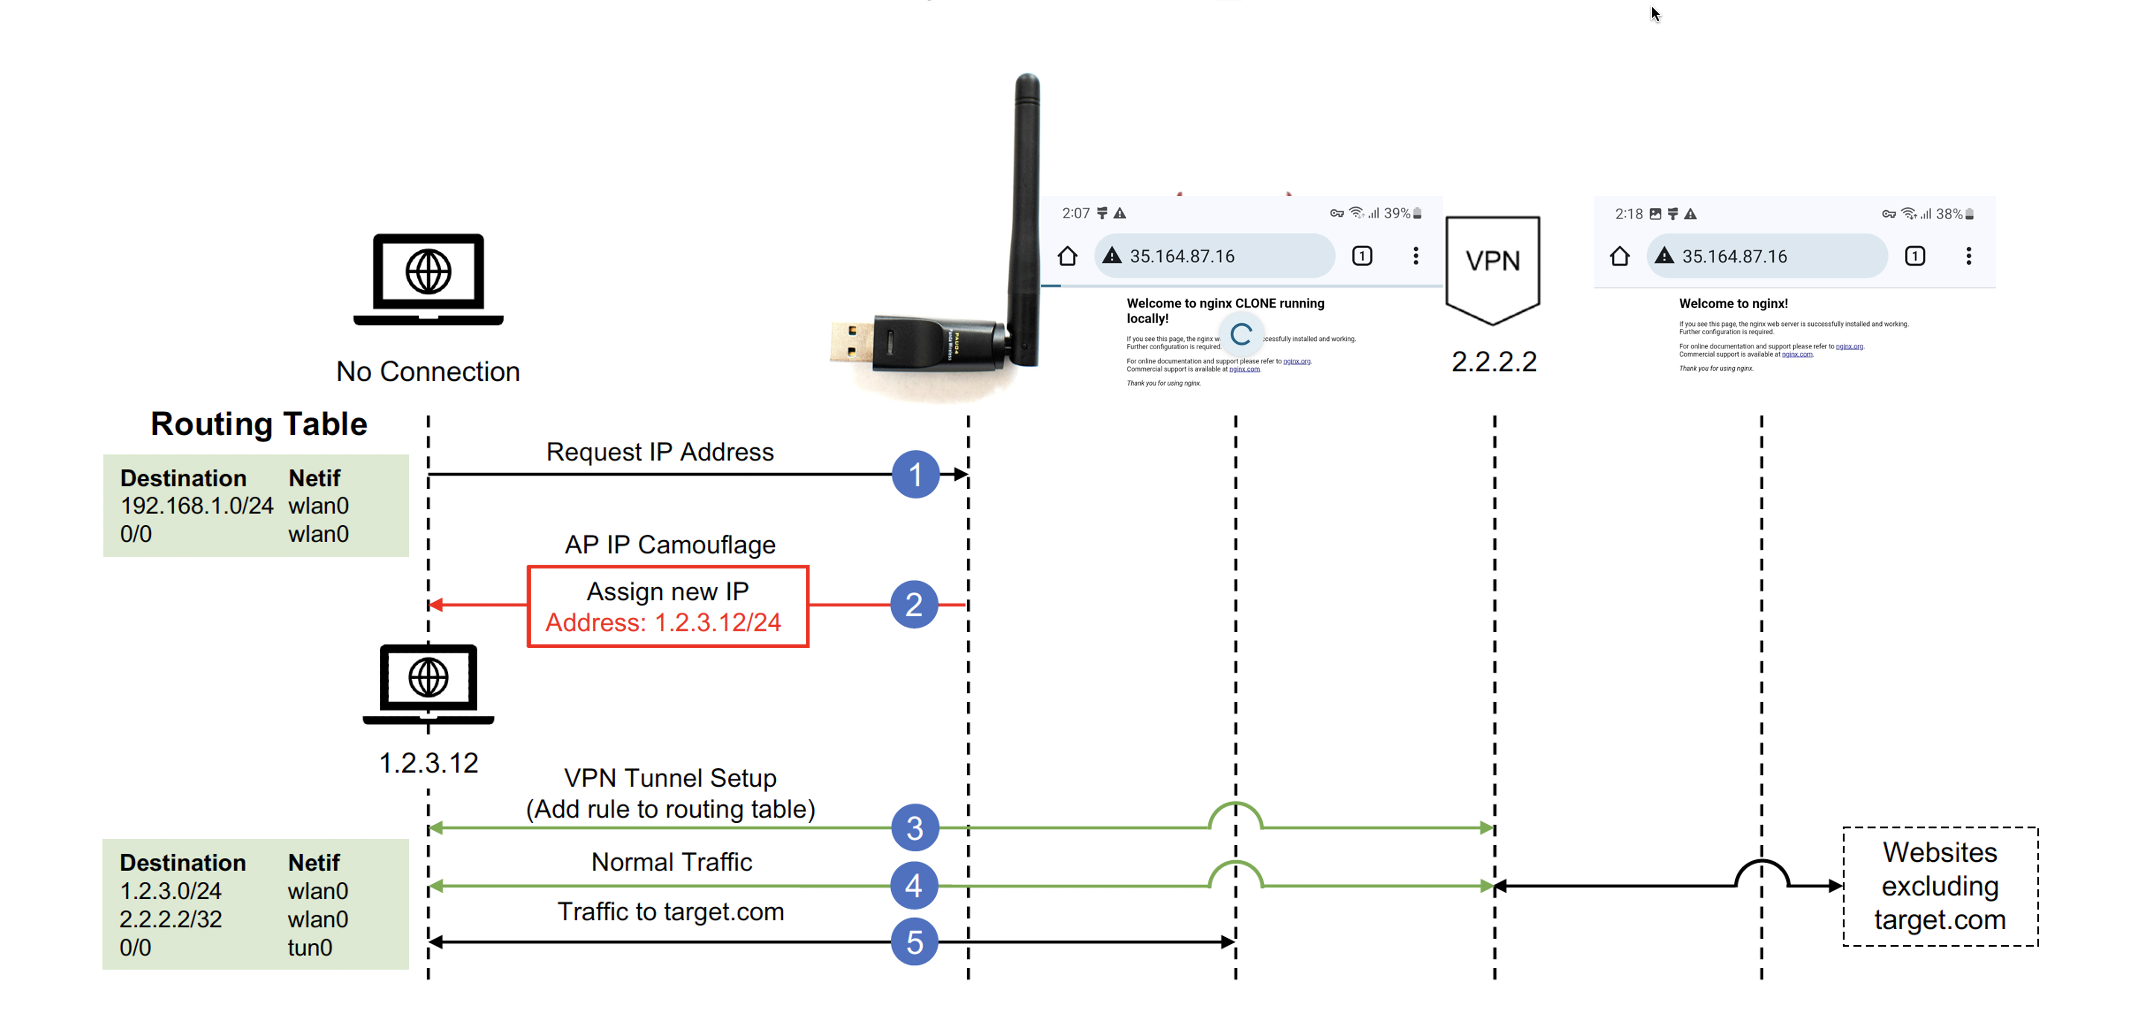
\includegraphics[width=\linewidth]{\images/mysetup}
	\caption{My experimental setup for LocalNet attack on VPN clients.}
	\label{fig:local-net-setup}
\end{figure}

For the ServerIP attack same setup has been used. But this time, in the rogue access point I also setup a DNS server to spoof DNS response from the VPN server.

\subsection{Test Subjects}
For the LocalNet Attack, I choose two VPN clients on 4 operating systems resulting in 8 test-subjects. 
\begin{enumerate}
	\item Hide.Me VPN \cite{hideme} on: iOS, Android, Windows, Mac
	\item Hotspot Shield VPN \cite{hotspotshield} on: iOS, Android, Windows, Mac
\end{enumerate}

For the ServerIP attack I tested built-in VPN clients on 3 operating systems (iOS, Android, Mac) with VPNGate \cite{vpngate} as the VPN server.
As mentioned in the paper \cite{vpnleaks}, none of the custom VPN clients is actually vulnerable to ServerIP attack.
The reason is custom VPN clients do not use DNS to find the IP address of the VPN server.
As a result, authors tried to test the built-in VPN clients with profiles from VPN servcice provider.
There was only one free VPN service provider which is VPNGate\cite{vpngate}.
When testing for ServerIP attacks, we look for plain text DNS queries in Wireshark \cite{wireshark}.
Because when connecting to VPN server, if the VPN client sends a DNS query in plain text,
then the client is vulnerable to ServerIP attack..

\section{Experimental Results}
Behavior of VPN clients under LocalNet attack or ServerIP attack can be categorized into these 4 categories:
\begin{itemize}
	\item Leaking: These VPN will leak traffic outside of VPN tunnel.
	\item Not Leaking: These VPN clients never leak traffic outside of VPN tunnel.
	\item Conditional Leaking: These VPN client leaks traffic if access to local network in enabled.
	\item Blocking: These VPN clients do not leak traffic outside of VPN client but blocks access to the target website.
\end{itemize}

I will explain result of LocalNet with Hotspot Shield VPN on Android and iOS. Rest of the results are presented in the table \ref{tab:local-net-summary}. 
\begin{table}[h]
    \centering
    \begin{tabular}{|p{40mm}|p{30mm}|p{75mm}|}
    \hline
    VPN(version) & Operating System  (version) & Result\\
     \hline
     \hline
     \hline
    Hotspot Shield (10.9.0) & Android (13)  & Not Leaking \\
    \hline
    Hotspot Shield (8.10.0) & iOS (17.1.2) & Leaking \\
    \hline
    Hotspot Shield (12.5.1) & Windows 10  &  Leaking \\
    \hline
    Hotspot Shield (6.5.0) & Mac (14.1) & Leaking \\
    \hline
    \hline
     Hide.Me(4.1.x) & Android (13)  & Leaking when local network connection is enabled. \\
     \hline
    Hide.Me(5.0.1) & iOS (17.1.2) & Leaking \\
    \hline
     Hide.Me(3.14.0) & Windows 10  &  Sends ARP request for targets IP then blocks local connection \\
    \hline
    Hide.Me(5.2.2) & Mac (14.1) & Leaking \\
    \hline
    \hline
    VPN Unlimited paid (9.1.19) & iOS 17.2.1 & Leaking \\
    \hline
    \end{tabular}
    \caption{Summary of LocalNet attack on 2 VPN clients: Hide.Me VPN and Hotspot Shield VPN }
    \label{tab:local-net-summary}
\end{table}
I will also explain ServerIP attack on iOS, remaining results are presented on table \ref{tab:server-ip-summary}.
\begin{table}
	\centering
	\begin{tabular}{|p{60mm}|p{40mm}|p{50mm}|}
		\hline
		VPN Client (Operating System) & Service Provider & Result \\
		\hline
		\hline
		\hline
		Built-in (iOS 17.1.2) & VPN Gate & Leaking \\
		\hline
		Built-in (Mac OS 14.1) & VPN Gate & Leaking \\
		\hline
		Android (13) & VPN Gate & Leaking \\
		\hline
	\end{tabular}
	\caption{Result of ServerIP attacks on built-in VPN clients on Mac, iOS and Android}
	\label{tab:server-ip-summary}
\end{table}


\subsection{LocalNet Attack on Hotspot Shield VPN 6.5.0 on Mac 14.1}
 Hotspot Shield VPN 6.5.0 on Mac OS 14.1 is vulnerable to LocalNet attack.
As we can see on \fig \ref{fig:hs-mac} VPN is connected using Hotspot Shield app.
When visiting our target website \href{}{http://35.164.87.16},
loaded web page does have ``CLONE'' mark in it.
Because browser is loading the website from the local nginx server.
\begin{figure*}[h]
	\centering
	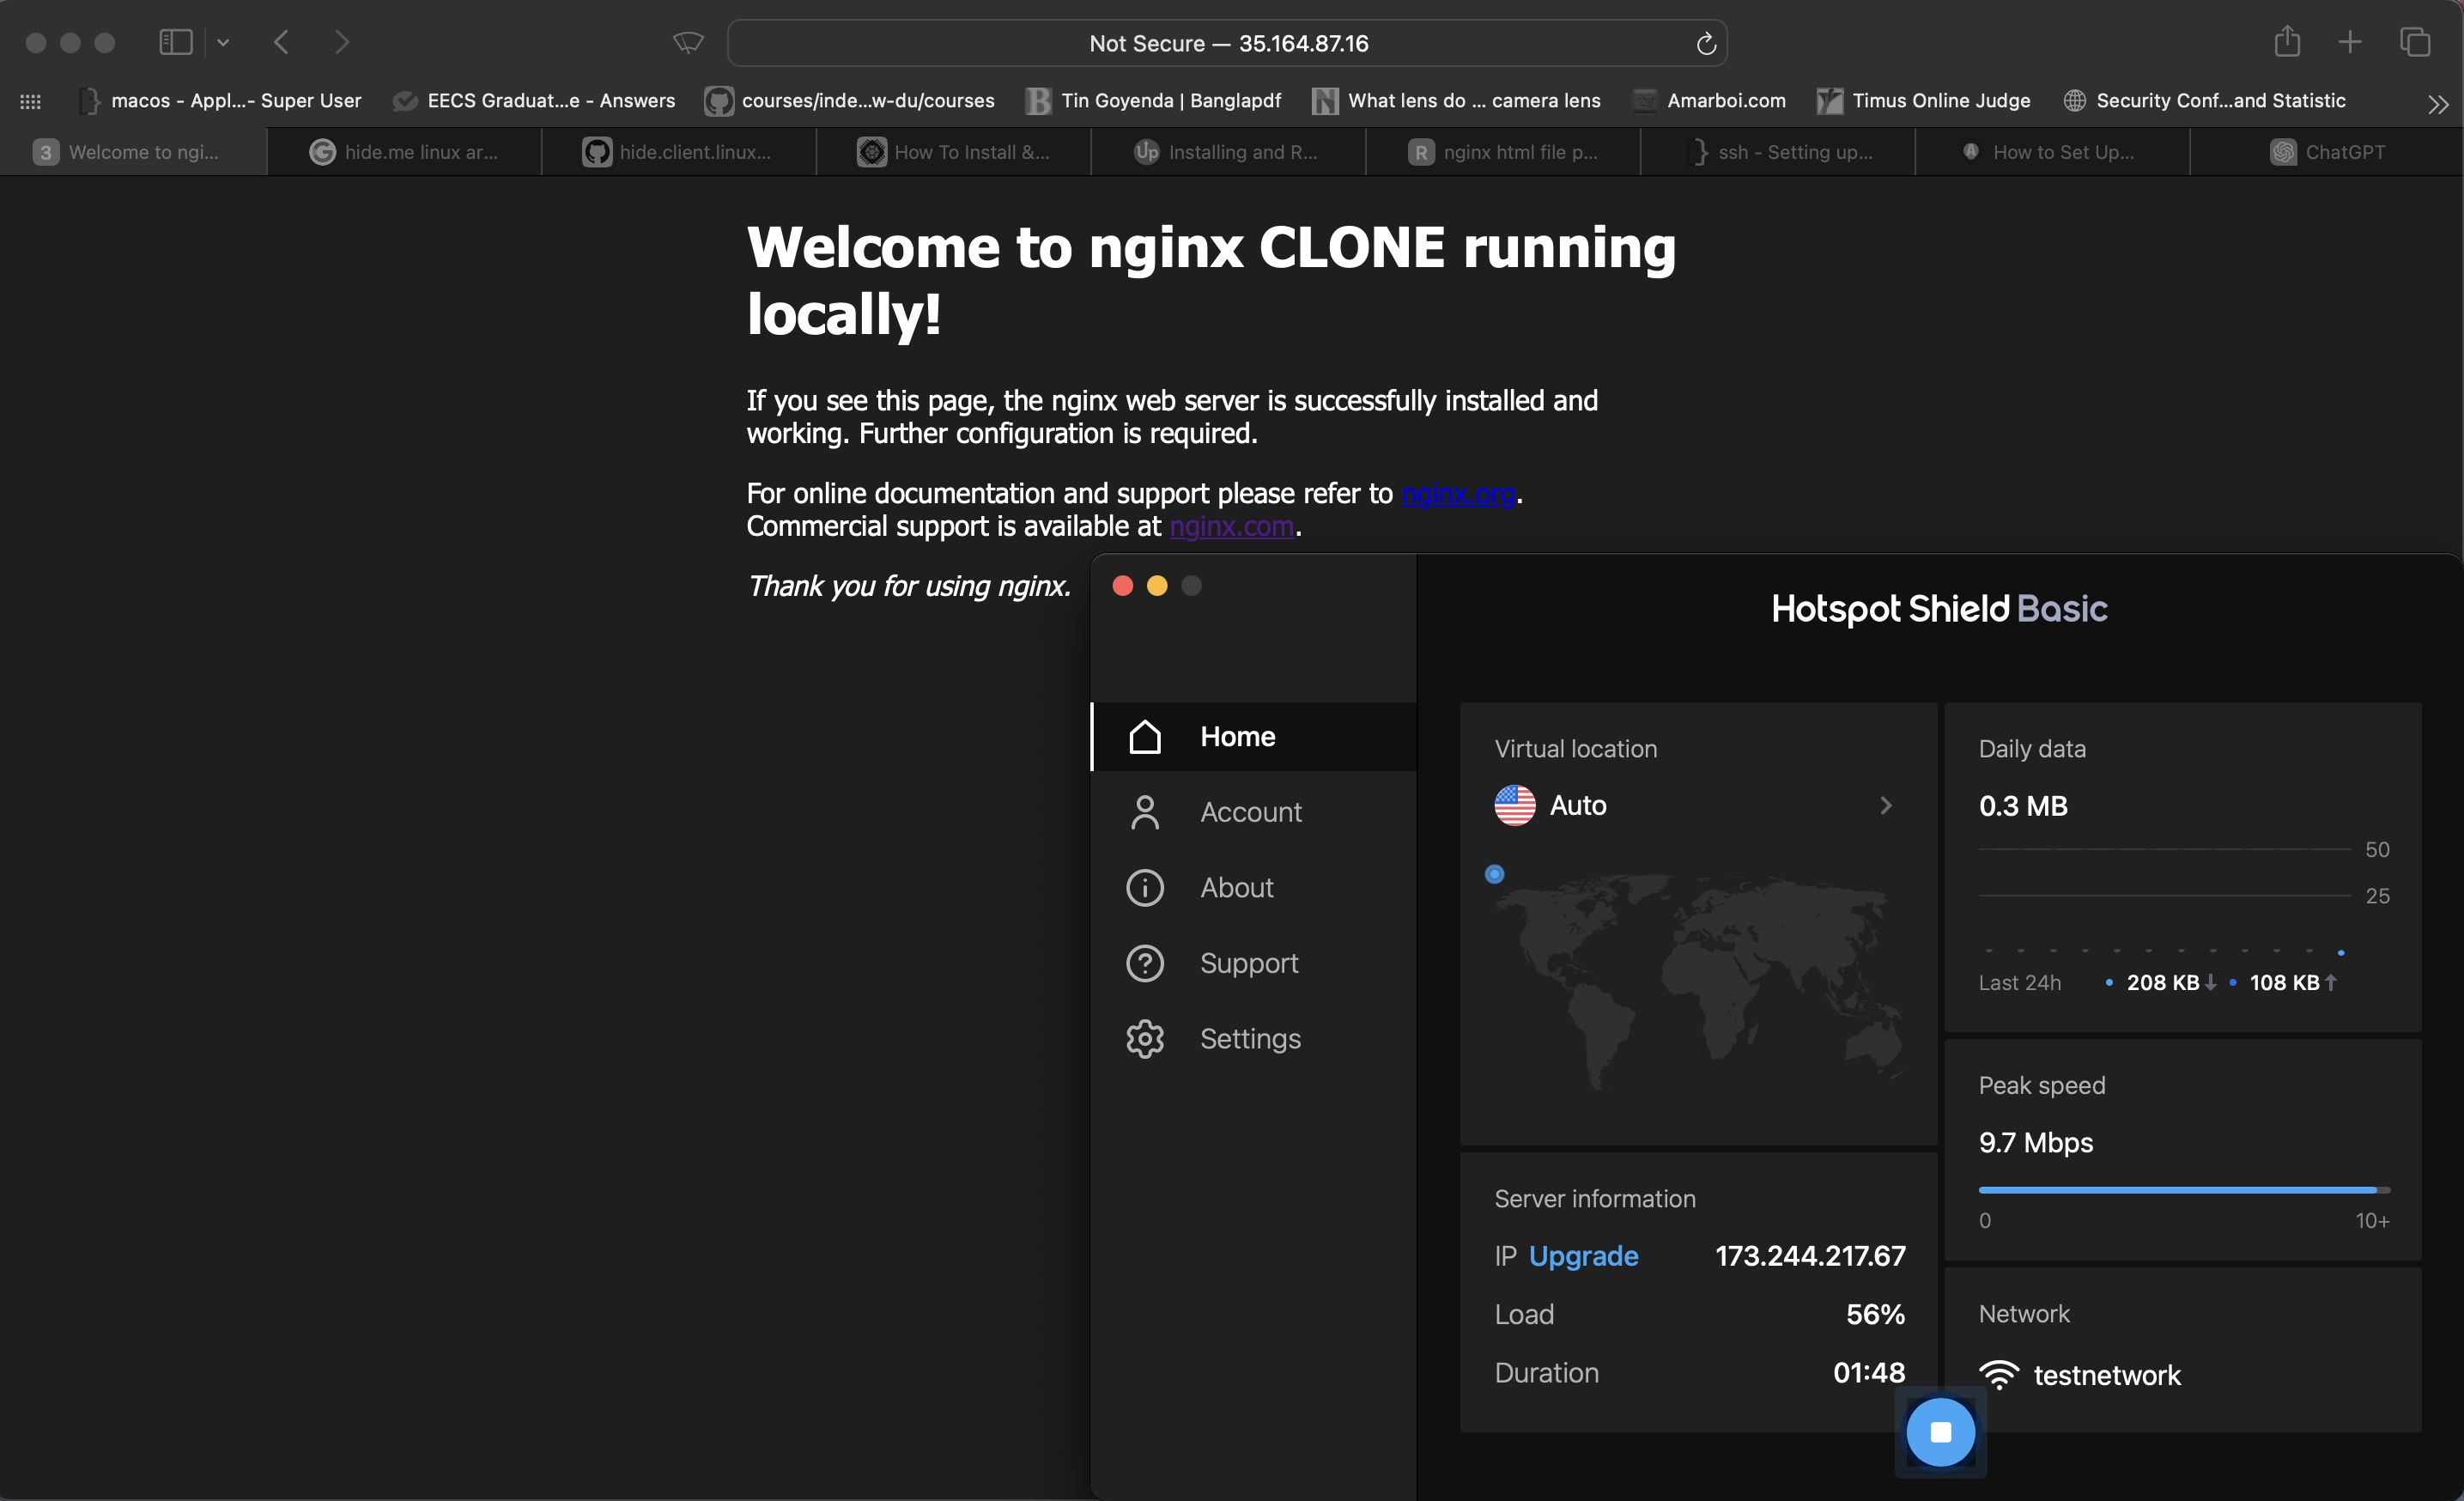
\includegraphics[width=\linewidth]{\images/hotspot-shield-mac-leaking.png}
	\caption{Hotspot Shield VPN on Mac in vulnerable to LocalNet attack}
	\label{fig:hs-mac}
\end{figure*}

\subsection{LocalNet Attack on Hotspot Shield VPN 10.9.0 on Android 13}
 Hotspot Shield VPN 10.9.0 on Android 13 is not vulnerable to LocalNet attack.
 As we can see on \fig \ref{fig:hs-andr} VPN is connected using Hotspot Shield app,
 on \fig \ref{fig:hs-andr-res} when visiting our target website \href{}{http://35.164.87.16},
 loaded web page does not have ``CLONE'' mark in it.
Because browser is loading the website from the public aws server.
\begin{figure*}[h!]
	\centering
	\begin{subfigure}{0.35\textwidth}
		\centering
		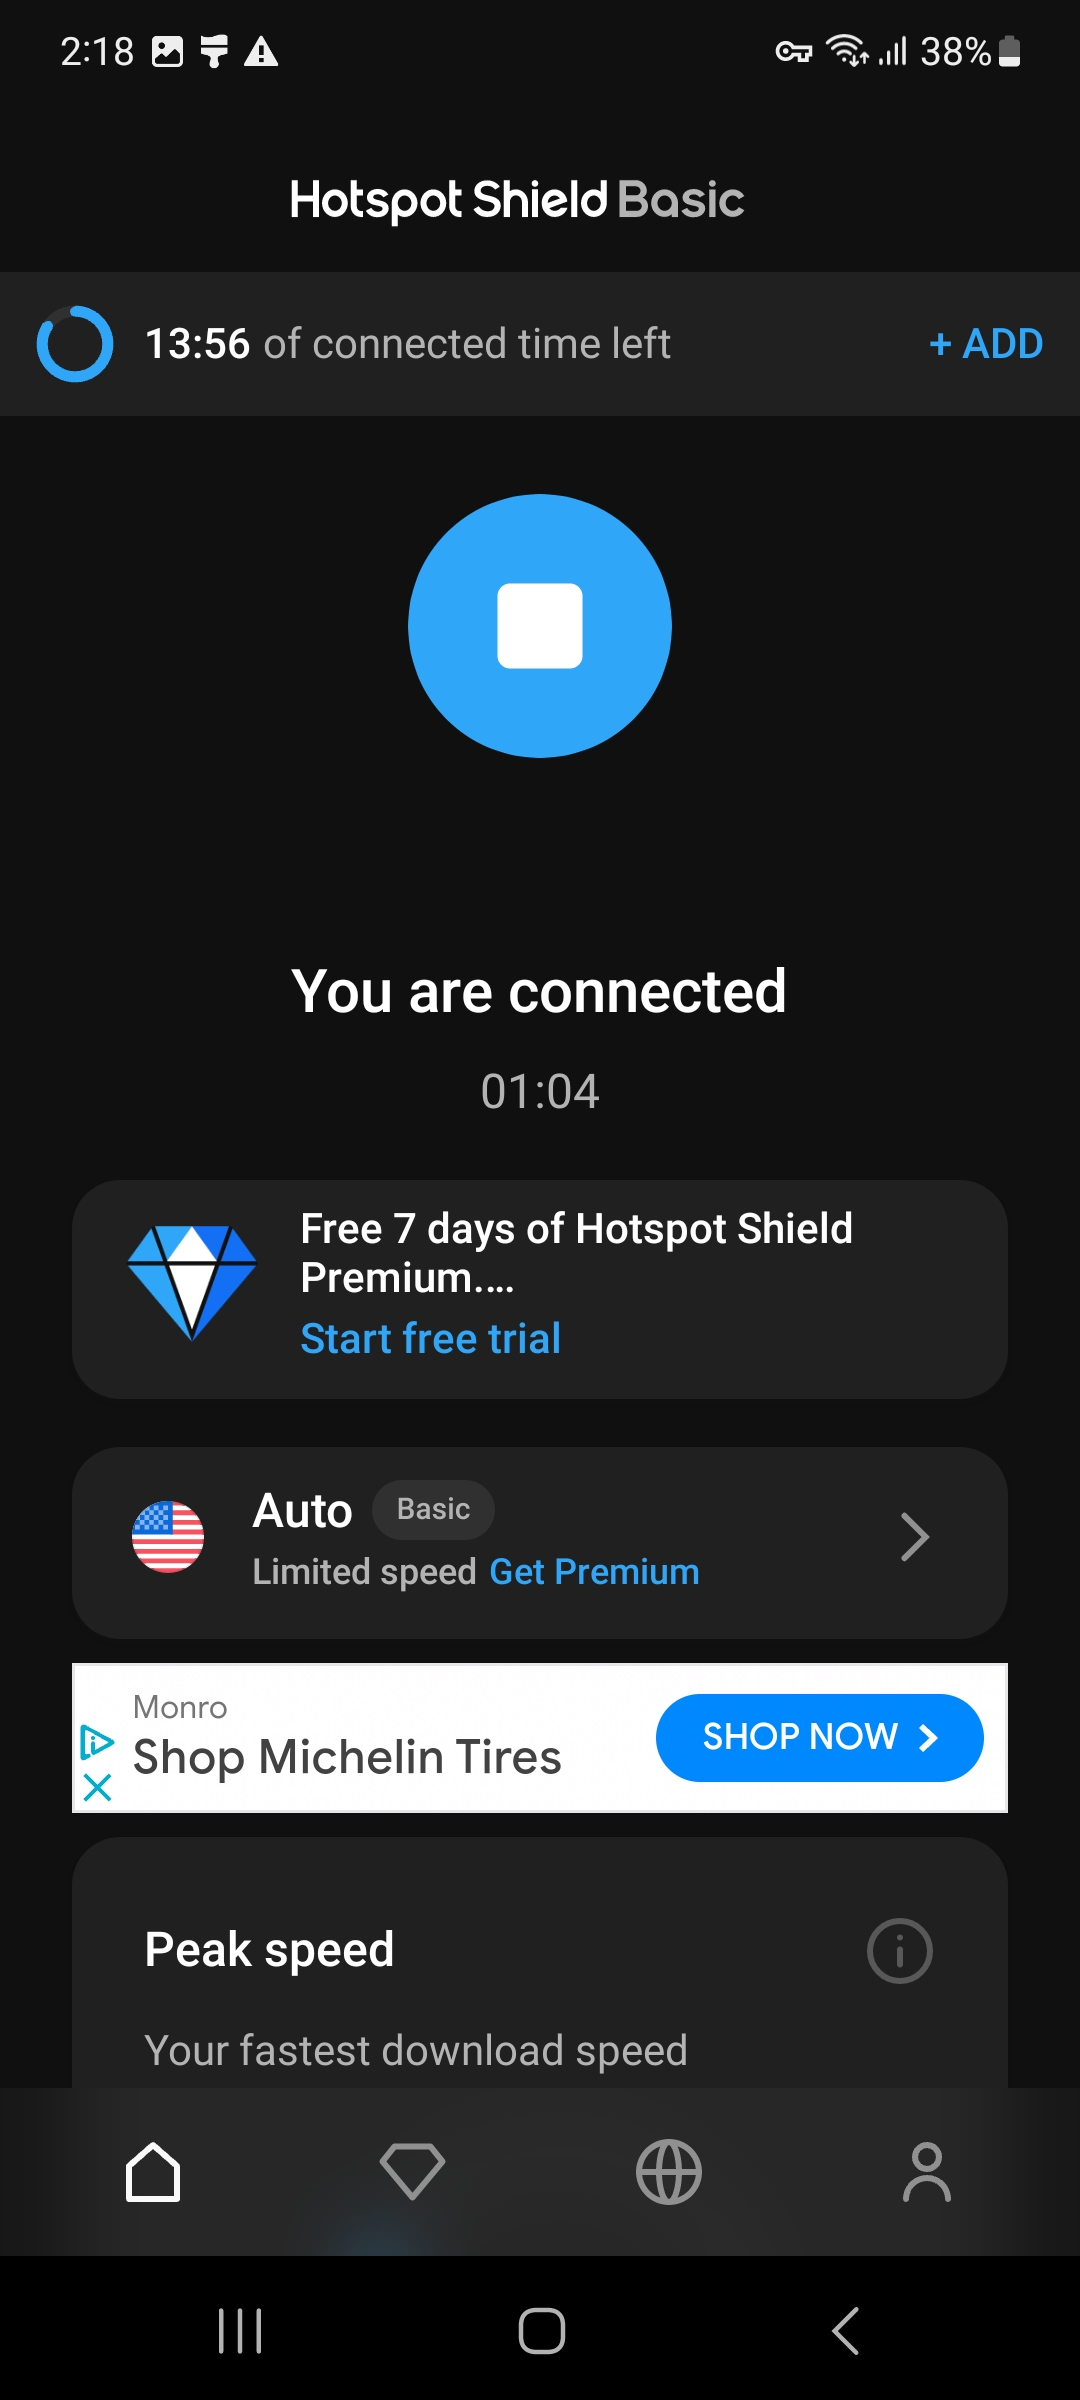
\includegraphics[width=\linewidth]{\images/Hotspot-Shield-andr-VPN.jpg}
		\caption{Hotspot Shield VPN app on Android}
		\label{fig:hs-andr}
	\end{subfigure}
	\begin{subfigure}{0.35\linewidth}
		\centering
		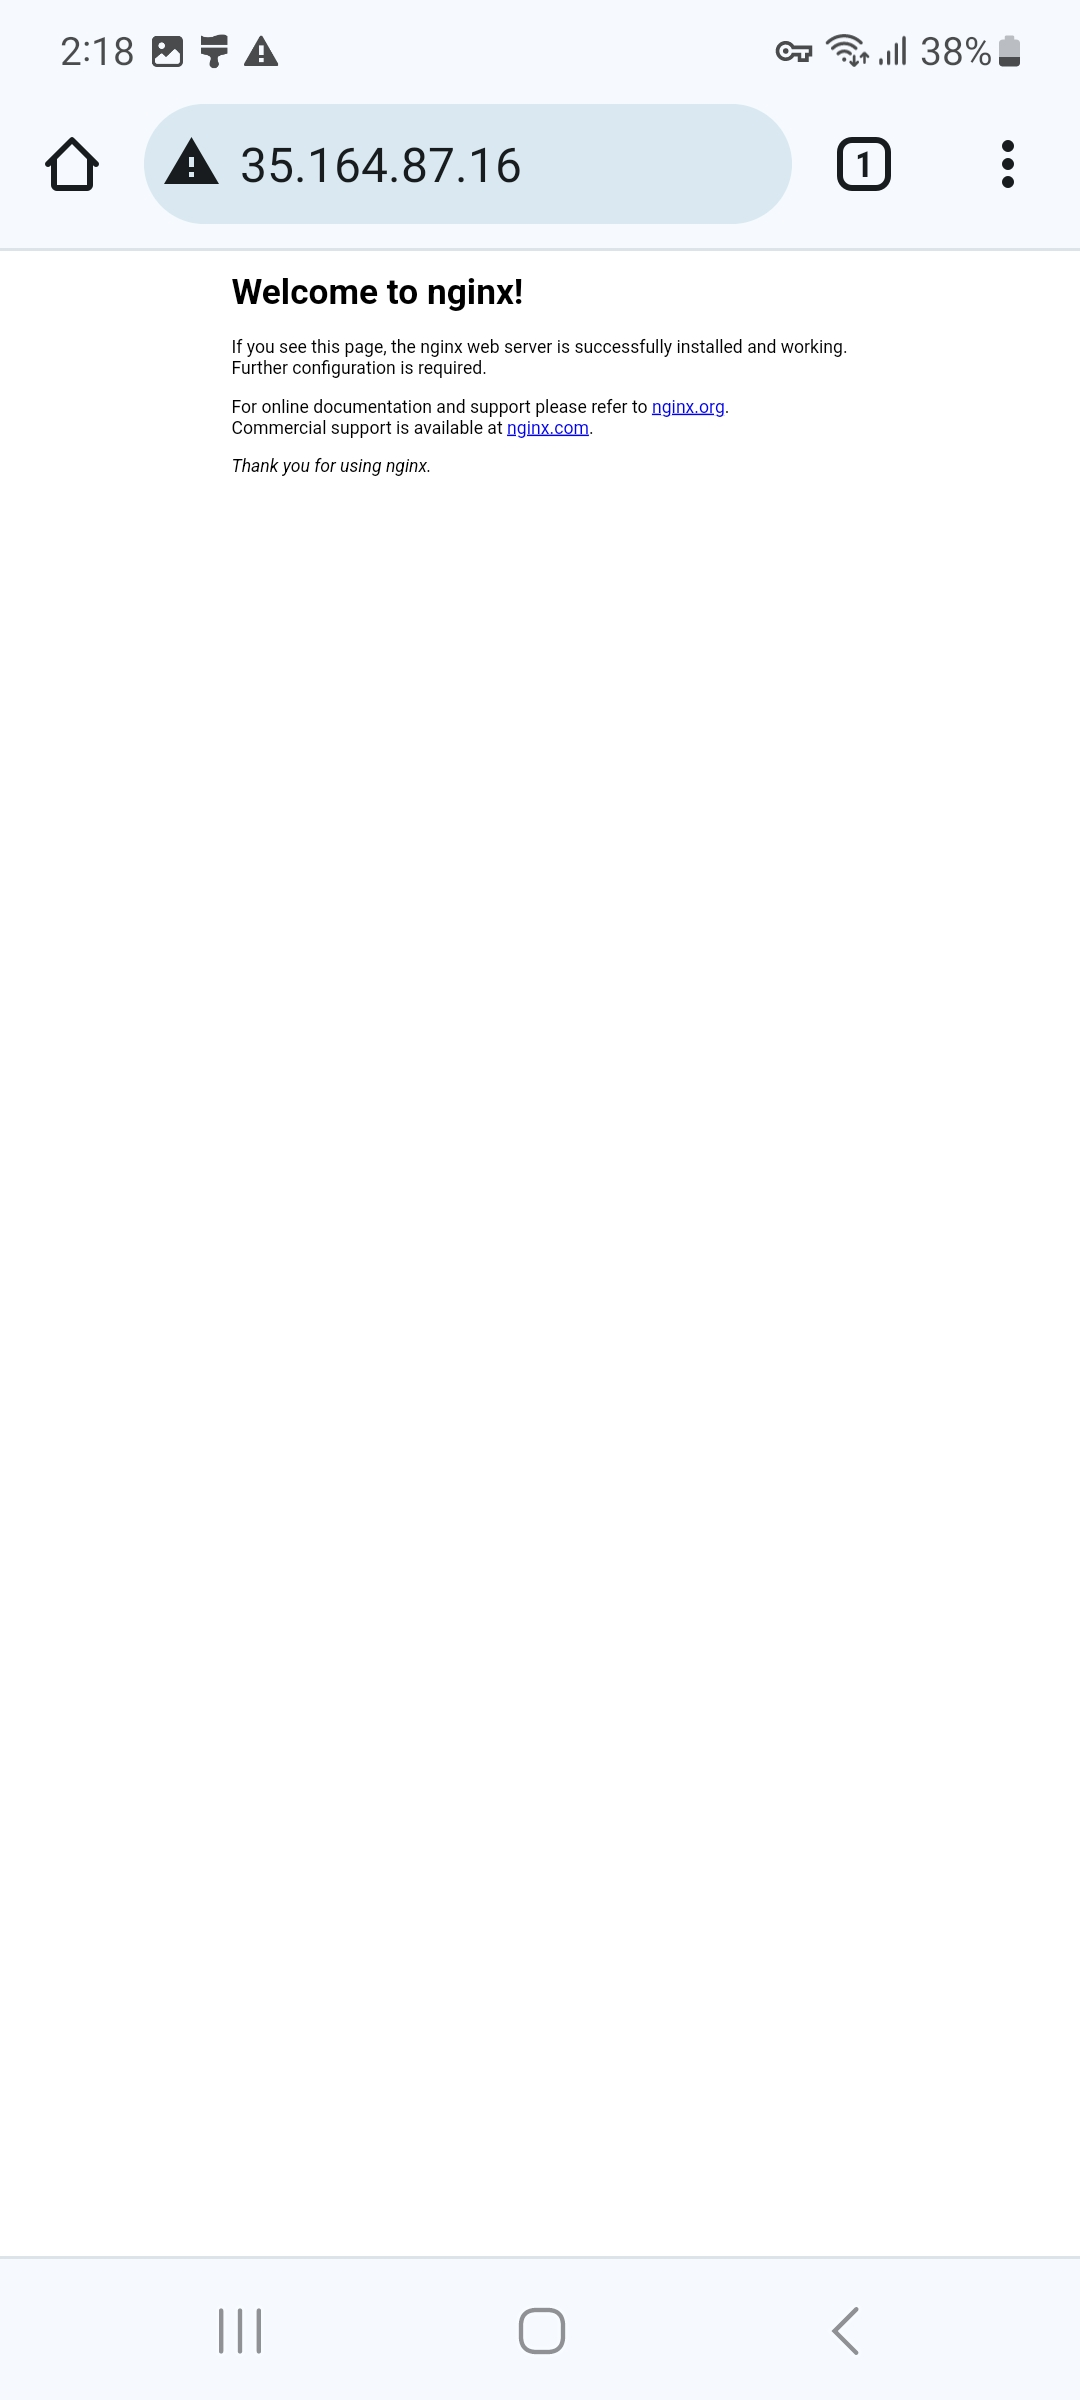
\includegraphics[width=\linewidth]{\images/Hotspot-Shield-andr-result.jpg}
		\caption{Loading target website  \href{}{http://35.164.87.16}}
		\label{fig:hs-andr-res}
	\end{subfigure}
	\caption{Testing Hotspot Shield VPN on Android for LocalNet attack}
	\label{fig:hs-andoird}
\end{figure*}

\subsection{ServerIP Attack on Built-In VPN clinet on iOS 17.1.2}
As shown in \fig \ref{fig:server-ip-ios} built-in VPN client of iOS 17.1.2 is connecting to VPN server of VPN-Gate.
At the same time, if we look at wireshark on \fig \ref{fig:server-ip-ios-res}, we can see a plain text DNS qwery for the IP address of VPN server.
Meaning, built-in VPN client of iOS 17.1.2 is vulnerable to ServerIP attack. Similar result has been noticed on Android and Mac.
\begin{figure*}[h]
	\centering
	\begin{subfigure}{0.20\textwidth}
		\centering
		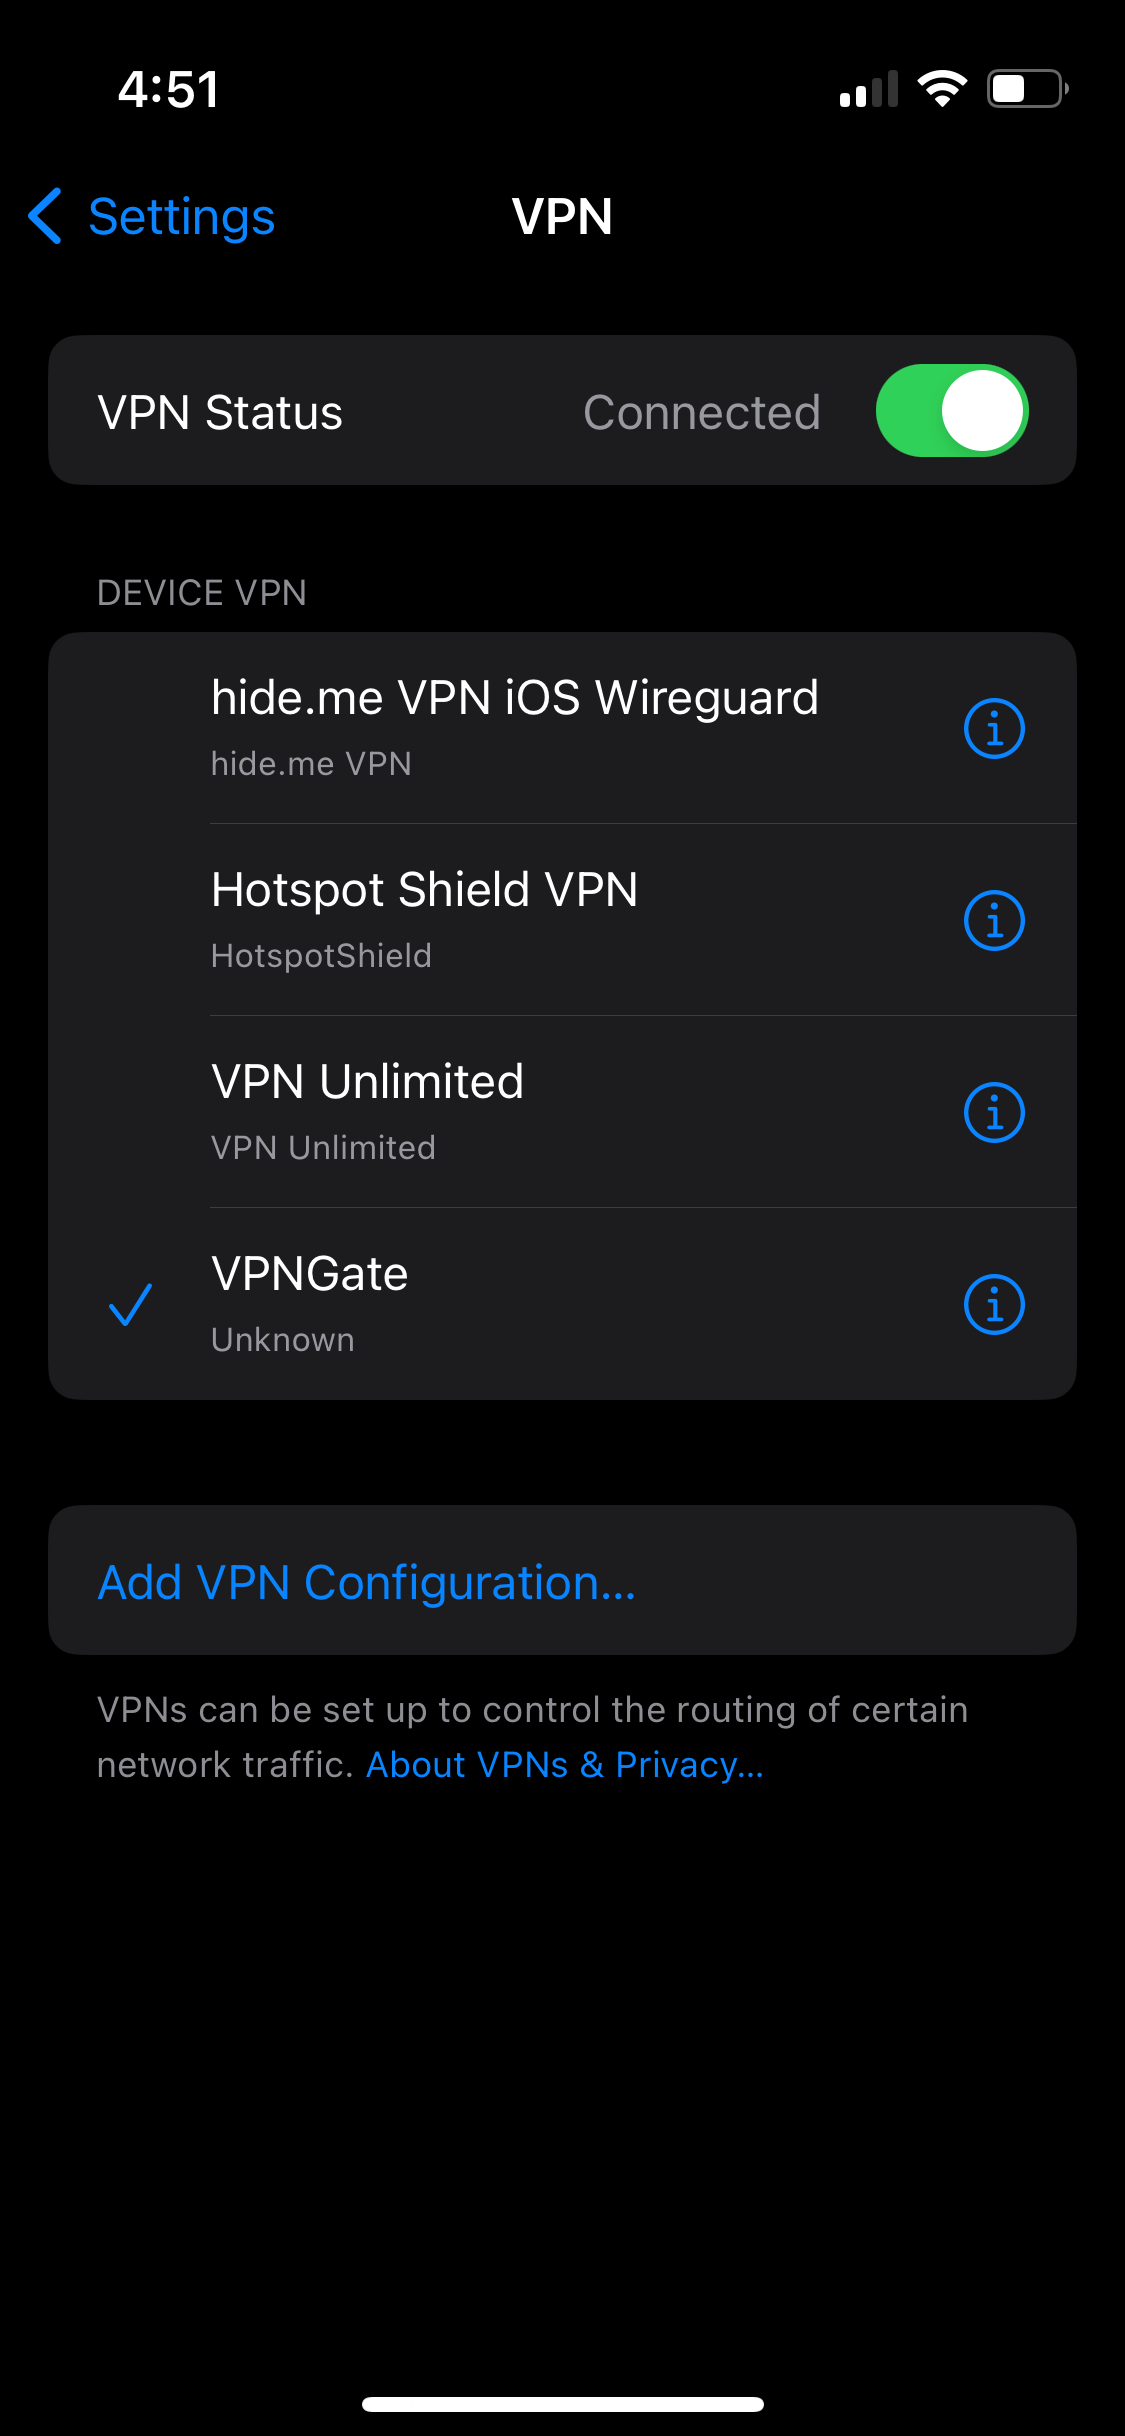
\includegraphics[width=\linewidth]{\images/server-ip-ios.PNG}
		\caption{Connecting to VPNGate with built in VPN client of iOS 17.2.1}
		\label{fig:server-ip-ios}
	\end{subfigure}
	\begin{subfigure}{0.75\textwidth}
		\centering
		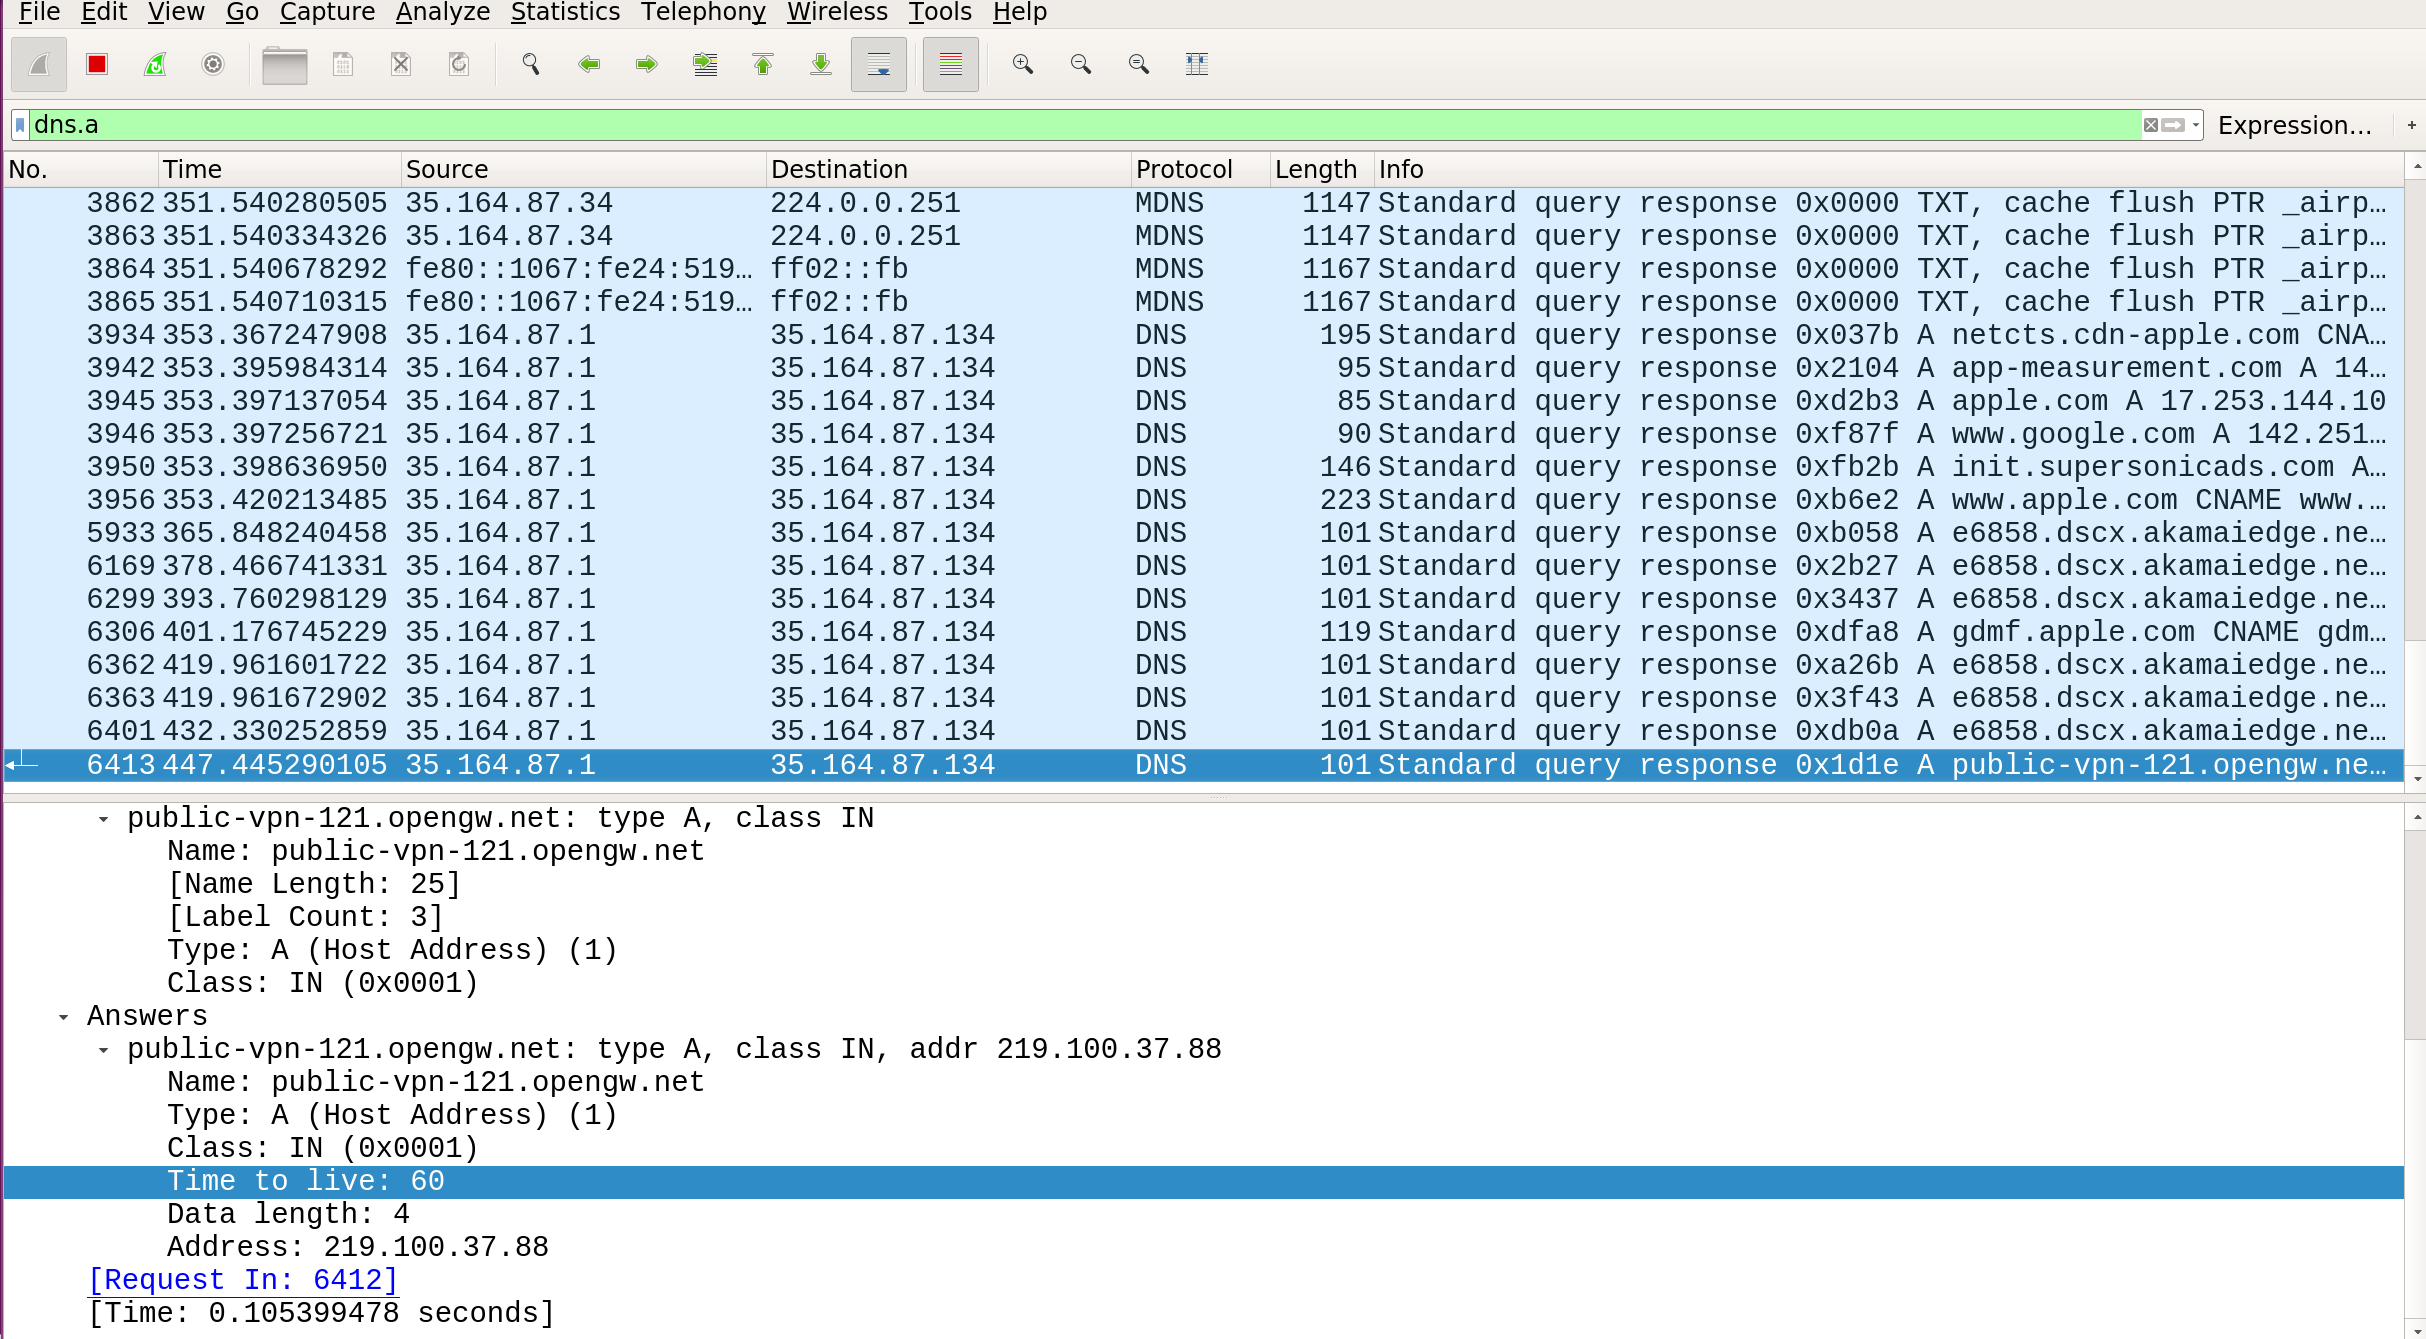
\includegraphics[width=\linewidth]{\images/dns-plain-qwery-ios.png}
		\caption{Plain text DNS query when connecting to VPN server of VPNGate}
		\label{fig:server-ip-ios-res}
	\end{subfigure}
	\caption{Testing built-in VPN client on iOS for ServerIP attack}
	\label{fig:server-ip}
\end{figure*}

\section{Discussion}
My goal on this project was to reproduce all categories of result presented in the paper \cite{vpnleaks}.
In the original paper, authors tested large number of VPN clients. Big number of those VPN clients were paid clients.
I tested only free VPN clients. I added one paid VPN client which I use for my personal usage.
That VPN client was also vulnerable to the attack.
In the end, I was actually able to reproduce results of all 4 categories.
% \begin{figure}[!h]
%     \centering
%     \begin{minipage}[b]{0.5\textwidth}
%         \includegraphics[width=\textwidth]{images/acl_Send_data.png}
%         \caption{ACL packet sending}
%     \end{minipage}
%   \hfill
%   \begin{minipage}[b]{0.4\textwidth}
%     \includegraphics[width=\textwidth]{images/acl_receive_data.png}
%     \caption{ACL packet receiving}
%   \end{minipage}
% \end{figure}

%\printbibliography
%\begin{}
%	content...
%\end{}
\bibliography{bibItem} 
\bibliographystyle{plainurl}
\end{document}
